% vim:ts=2 sw=2 et:

% main.tex -- Paper zum Thema <kugel>
%
% (c) 2020 Hochschule Rapperswil
%
\chapter{Spherical Harmonics\label{chapter:kugel}}
\lhead{Spherical Harmonics}
\rhead{Long Proofs}
\begin{otherlanguage}{english}
\begin{refsection}
\chapterauthor{Manuel Cattaneo and Naoki Pross}

% vim:ts=2 sw=2 et spell tw=78:

\section{Introduction}

This chapter of the book is devoted to the sef of functions called
\emph{spherical harmonics}. However, before we dive into the topic, we want to
make a few preliminary remarks to avoid ``upsetting'' a certain type of
reader. Specifically, we would like to specify that the authors of this
chapter are not mathematicians but engineers, and therefore the text will not be
always complete with sound proofs after every claim. Instead we will go
through the topic in a more intuitive way including rigorous proofs only if
they are enlightening or when they are very short. Where no proofs are given
we will try to give an intuition for why it is true.

That being said, when talking about spherical harmonics one could start by
describing their name. The latter may be a cause of some confusion because of
the misleading translations in other languages. In German the name for this
set of functions is ``Kugelfunktionen'', which puts the emphasis only on the
spherical context, whereas the English name ``spherical harmonics'' also
contains the \emph{harmonic} part hinting at Fourier theories and harmonic
analysis in general.

The structure of this chapter is organized in the following way. First, we
will quickly go through some fundamental linear algebra and Fourier theory to
refresh a few important concepts. In principle, we could have written the
whole thing starting from a much more abstract level without much preparation,
but then we would have lost some of the beauty that comes from the
appreciation of the power of some surprisingly simple ideas. Then once the
basics are done, we can explore the main topic of spherical harmonics which as
we will see arises from the eigenfunctions of the Laplacian operator in
spherical coordinates. Finally, after studying what we think are the most
beautiful and interesting properties of the spherical harmonics, to conclude
this journey we will present a few real-world applications, which are of
course most of interest for engineers.


% vim:ts=2 sw=2 et spell tw=78:

\section{Preliminaries}\label{kugel:sec:preliminaries}

The purpose of this section is to dust off some concepts that will become
important later on. This will enable us to get a richer and more general view
of the topic rather than just liming ourselves to a specific example.
However, if the reader is already very familiar with the following concepts:
inner product space, Hilbert space, Fourier series, Laplacian operator and
eigenvalue problems, this entire section may be skipped.

\subsection{Inner Product Spaces}

We shall start with a few fundamentals of linear algebra. We will mostly work
with complex numbers, but for the sake of generality we will do what most
textbook do, and write \(\mathbb{K}\) instead of \(\mathbb{C}\) since the
theory works the same when we replace \(\mathbb{K}\) with the real
numbers \(\mathbb{R}\).

\if 0
\begin{definition}[Vector space]
  \label{kugel:def:vector-space} \nocite{axler_linear_2014}
  A \emph{vector space} over a field \(\mathbb{K}\) is a set \(V\) with an
  addition on \(V\) and a multiplication on \(V\) such that the following
  properties hold:
  \begin{enumerate}[(a)]
    \item (Commutativity) \(u + v = v + u\) for all \(u, v \in V\);
    \item (Associativity) \((u + v) + w = u + (v + w)\) and \((ab)v = a(bv)\)
      for all \(u, v, w \in V\) and \(a, b \in \mathbb{K}\);
    \item (Additive identity) There exists an element \(0 \in V\) such that
      \(v + 0 = v\) for all \(v \in V\);
    \item (Additive inverse) For every \(v \in V\), there exists a \(w \in V\)
      such that \(v + w = 0\);
    \item (Multiplicative identity) \(1 v = v\) for all \(v \in V\);
    \item (Distributive properties) \(a(u + v) = au + av\) and \((a + b)v = av +
      bv\) for all \(a, b \in \mathbb{K}\) and all \(u,v \in V\).
  \end{enumerate}
\end{definition}

\begin{definition}[Dot product]
  \label{kugel:def:dot-product}
  In the vector field \(\mathbb{K}^n\) the scalar or dot product between two
  vectors \(u, v \in \mathbb{K}^n\) is
  \(
    u \cdot v 
    = u_1 \overline{v}_1 + u_2 \overline{v}_2 + \cdots + u_n \overline{v}_n
    = \sum_{i=1}^n u_i \overline{v}_i.
  \)
\end{definition}

\kugeltodo{Text here.}

\begin{definition}[Span]
\end{definition}

\kugeltodo{Text here.}

\begin{definition}[Linear independence]
\end{definition}


\kugeltodo{Text here.}

\begin{definition}[Basis]
\end{definition}

\kugeltodo{Text here.}
\fi

\begin{definition}[Inner product]
  \label{kugel:def:inner-product} \nocite{axler_linear_2014}
  The \emph{inner product} on \(V\) is a function that takes each ordered pair
  \((u, v)\) of elements of \(V\) to a number \(\langle u, v \rangle \in
  \mathbb{K}\) and has the following properties:
  \begin{enumerate}[(a)]
    \item (Positivity) \(\langle v, v \rangle \geq 0\) for all \(v \in V\);
    \item (Definiteness) \(\langle v, v \rangle = 0\) iff \(v = 0\);
    \item (Additivity) \(
        \langle u + v, w \rangle =
        \langle u, w \rangle + \langle v, w \rangle
      \) for all \(u, v, w \in V\);
    \item (Homogeneity) \(
        \langle \lambda u, v \rangle =
        \lambda \langle u, v \rangle
      \) for all \(\lambda \in \mathbb{K}\) and all \(u, v \in V\);
    \item (Conjugate symmetry)
      \(\langle u, v \rangle = \overline{\langle v, u \rangle}\) for all
      \(u, v \in V\).
  \end{enumerate}
\end{definition}

The inner product is a generalization of the scalar product that does not
explicitly depend on rows or columns of vectors. This has the interesting
consequence that anything that behaves according to the rules given in
definition \ref{kugel:def:inner-product} \emph{is} an inner product. For
example if we say that the vector space \(V = \mathbb{R}^n\), then the dot
product
\(
  u \cdot v = u_1 \overline{v}_1
    + u_2 \overline{v}_2
    + \cdots + u_n \overline{v}_n
\)
is an inner product in \(V\), and the two are said to form an \emph{inner
product space}.

\begin{definition}[Inner product space]
  \nocite{axler_linear_2014}
  An inner product space is a vector space \(V\) equipped with an inner
  product on \(V\).
\end{definition}

How about a more interesting example: the set of continuous complex valued
functions on $\mathbb{R}$ can behave like vectors.  Functions can be added,
subtracted, multiplied with scalars, are associative and there is even the
identity element (zero function \(f(x) = 0\)), so we can create an inner
product
\[
  \langle f, g \rangle = \int_\mathbb{R} f(x) \overline{g(x)} \, dx,
\]
which will indeed satisfy all of the rules for an inner product (in fact this
is called the Hermitian inner product\nocite{allard_mathematics_2009}). If
this last step sounds too easy to be correct, you are right, because it is not
quite so simple. The problem that we have swept under the rug here is
convergence, which any student who took an analysis class will know is a
rather hairy question. We will not need to go too much into the details since
formally discussing convergence is definitely beyond the scope of this text,
however, for our purposes we will still need to dig a little deeper for a few
more paragraph.

\subsection{Convergence}

In the last section we hinted that we can create ``infinite-dimensional''
vector spaces using functions as vectors, and inner product spaces by
integrating the product of two functions of said vector space. However, there
is a problem with convergence which twofold: the obvious problem is that the
integral of the inner product may not always converge, while the second is a
bit more subtle and will be discussed later. The inner product that does
not converge is a problem because we want a \emph{norm}.

\begin{definition}[\(L^2\) Norm]
  \nocite{axler_linear_2014}
  The norm of a vector \(v\) of an inner product space is a number
  denoted as \(\| v \|\) that is computed by \(\| v \| = \sqrt{\langle v, v
  \rangle}\).
\end{definition}

In \(\mathbb{R}^n\) with the dot product (Euclidian space) the norm is the
geometric length of a vector, while in a more general inner product space the
norm can be thought of as a more abstract measure of ``length''. In any case
it is rather important that the expression \(\sqrt{\langle v, v \rangle}\),
which when using functions \(f: \mathbb{R} \to \mathbb{C}\) becomes
\[
  \sqrt{\langle f, f \rangle} =
  \sqrt{\int_\mathbb{R} f(x) \overline{f(x)} \, dx} =
  \sqrt{\int_\mathbb{R} |f(x)|^2 \, dx},
\]
always exists. So, to fix this problems we do what mathematicians do best:
make up the solution. Since the integrand under the square root is always the
square of the magnitude, we can just specify that the functions must be
\emph{absolutely square integrable}. To be more compact it is common to just
write \(f \in L^2\), where \(L^2\) denotes the set of absolutely square
integrable functions.

Now we can tackle the second (much more difficult) problem of convergence
mentioned at the beginning. Using the technical jargon, we need that our inner
product space is what is called a \emph{complete metric space}, which just
means that we can measure distances. For the more motivated readers although
not really necessary we can also give a more formal definition, the others can
skip to the end of the section where there is definition
\ref{kugel:def:hilbert}.

\begin{definition}[Metric space]
  \nocite{tao_analysis_2016}
  A metric space \((X, d)\) is a space \(X\) of objects (called points),
  together with a distance function or metric \(d: X \times X \to [0,
  +\infty)\), which associates to each pair \(x, y\) of points in \(X\) a
  non-negative real number \(d(x, y) \geq 0\). Furthermore, the metric must
  satisfy the following four axioms:
  \begin{enumerate}[(a)]
    \item For any \(x\in X\), we have \(d(x, x) = 0\).
    \item (Positivity) For any \emph{distinct} \(x, y \in X\), we have
      \(d(x,y) > 0\).
    \item (Symmetry) For any \(x,y \in X\), we have \(d(x, y) = d(y, x)\).
    \item (Triangle inequality) For any \(x, y, z \in X\) we have
      \(d(x, z) \leq d(x, y) + d(y, z)\).
  \end{enumerate}
\end{definition}

As is seen in the definition metric spaces are a very abstract concept and
rely on rather weak statements, which makes them very general. Now, the more
intimidating part is the \emph{completeness} which is defined as follows.

\begin{definition}[Complete metric space]
  \label{kugel:def:complete-metric-space}
  A metric space \((X, d)\) is said to be \emph{complete} iff every Cauchy
  sequence in \((X, d)\) is convergent in \((X, d)\).
\end{definition}

To fully explain definition \ref{kugel:def:complete-metric-space} it would
take a few more pages, which would get a bit too heavy. So instead we will
give an informal explanation through an counterexample to get a feeling of
what is actually happening. Cauchy sequences is a rather fancy name for a
sequence for example of numbers that keep changing, but in a such a way that
at some point the change keeps getting smaller (the infamous
\(\varepsilon-\delta\) definition). For example consider the sequence of
numbers
\[
  1,
  1.4,
  1.41,
  1.414,
  1.4142,
  1.41421,
  \ldots
\]
in the metric space \((\mathbb{Q}, d)\) with \(d(x, y) = |x - y|\). Each
element of this sequence can be written with some fraction in \(\mathbb{Q}\),
but in \(\mathbb{R}\) the sequence is converging towards the number
\(\sqrt{2}\). However, \(\sqrt{2} \notin \mathbb{Q}\). Since we can find a
sequence of fractions whose distance's limit is not in \(\mathbb{Q}\), the
metric space \((\mathbb{Q}, d)\) is \emph{not} complete. Conversely,
\((\mathbb{R}, d)\) is a complete metric space since \(\sqrt{2} \in
\mathbb{R}\).

Of course the analogy above also applies to vectors, i.e. if in an inner
product space \(V\) over a field \(\mathbb{K}\) all sequences of vectors have
a distance that is always in \(\mathbb{K}\), then \(V\) is also a complete
metric space. In the jargon, this particular case is what is known as a
Hilbert space, after the very influential German mathematician David Hilbert.

\begin{definition}[Hilbert space]
  \label{kugel:def:hilbert}
  A Hilbert space is a vector space \(H\) with an inner product \(\langle f, g
  \rangle\) and a norm \(\sqrt{\langle f, f \rangle}\) defined such that \(H\)
  turns into a complete metric space.
\end{definition}

\subsection{Orthogonal basis and Fourier series}
\label{kugel:sec:preliminaries:ortho-fourier}

Now we have almost everything we need to get into the domain of Fourier theory
from the perspective of linear algebra. However, we still need to briefly
discuss the matters of orthogonality\footnote{See chapter
\ref{buch:chapter:orthogonalitaet} for more on orthogonality.} and
periodicity. Both should be very straightforward and already well known.

\begin{definition}[Orthogonality and orthonormality]
  \label{kugel:def:orthogonality}
  In an inner product space \(V\) two vectors \(u, v \in V\) are said to be
  \emph{orthogonal} if \(\langle u, v \rangle = 0\). Further, if both \(u\)
  and \(v\) are of unit length, i.e. \(\| u \| = 1\) and \(\| v \| = 1\), then
  they are said to be ortho\emph{normal}.
\end{definition}

\begin{definition}[1-periodic function and \(C(\mathbb{R}/\mathbb{Z}; \mathbb{C})\)]
  A function is said to be 1-periodic if \(f(x + 1) = f(x)\). The set of
  1-periodic function from the real to the complex
  numbers is denoted by \(C(\mathbb{R}/\mathbb{Z}; \mathbb{C})\).
\end{definition}

In the definition above the notation \(\mathbb{R}/\mathbb{Z}\) was borrowed
from group theory, and is what is known as a quotient group; Not really
relevant for our discussion but still a ``good to know''. More importantly, it
is worth noting that we could have also defined more generally \(T\)-periodic
functions with \(L\in\mathbb{R}\), however, this would introduce a few ugly
\(T\)'s everywhere which are not really necessary (it will always be possible
to extend the theorems to \(\mathbb{R} / T\mathbb{Z}\)). Thus, we will
continue without the \(T\)'s, and to simplify the language unless specified
otherwise ``periodic'' will mean 1-periodic. Having said that, we can
officially begin with the Fourier theory.

\begin{lemma}
  \label{kugel:thm:sqint-hilbert}
  The subset of absolutely square integrable functions in
  \(C(\mathbb{R}/\mathbb{Z}; \mathbb{C})\) together with the Hermitian inner
  product
  \[
    \langle f, g \rangle = \int_{[0; 1)} f(x) \overline{g(x)} \, dx
  \]
  form a Hilbert space.
\end{lemma}
\begin{proof}
  It is not too difficult to show that the functions in \(C(\mathbb{R} /
  \mathbb{Z}; \mathbb{C})\) are well behaved and form a vector space. Thus,
  what remains is that the norm needs to form a complete metric space.
  However, this follows from the fact that we defined the functions to be
  absolutely square integrable\footnote{For the curious on why, it is because
  \(L^2\) is what is known as a \emph{compact metric space}, and compact
  metric spaces are always complete (see \cite{eck_metric_2022,
  tao_analysis_2016}). To explain compactness and the relationship between
  compactness and completeness is definitely beyond the goals of this text.}.
\end{proof}

This was probably a not very satisfactory proof since we brushed off a lot of
details by referencing other theorems. However, the main takeaway should be
that we have ``constructed'' this new Hilbert space of functions in a such a
way that from now on we will not have to worry about the fussy details of
convergence. Instead of worrying about convergence, we will use right away
this new Hilbert space.

\begin{lemma}
  \label{kugel:thm:exp-1d}
  The set of functions \(E_n(x) = e^{i2\pi nx}\) on the interval
  \([0; 1)\) with \(n \in \mathbb{Z} \) are orthonormal.
\end{lemma}
\begin{proof}
  We need to show that \(\langle E_m, E_n \rangle\) equals 1 when \(m = n\)
  and zero otherwise. This is a straightforward computation: We start by
  unpacking the notation to get
  \[
    \langle E_m, E_n \rangle
    = \int_0^1 e^{i2\pi mx} e^{- i2\pi nx} \, dx
    = \int_0^1 e^{i2\pi (m - n)x} \, dx,
  \]
  then inside the integrand we can see that when \(m = n\) we have \(e^0 = 1\) and
  thus \( \int_0^1 dx = 1, \) while when \(m \neq n\) we can just say that we
  have a new non-zero integer
  \(k := m - n\) and
  \[
    \int_0^1 e^{i2\pi kx} \, dx
    = \frac{e^{i2\pi k} - e^{0}}{i2\pi k}
    = \frac{1 - 1}{i2\pi k}
    = 0
  \]
  as desired. \qedhere
\end{proof}

Now, this is an useful lemma, because this set of orthonormal functions can be
used as basis of our Hilbert space of square integrable functions in
$C(\mathbb{R}/\mathbb{Z}; \mathbb{C})$, and the interesting consequence is the
fact that we can create linear combinations of these basis functions to obtain
other functions. This was Fourier's insight: any reasonable function can be
expressed using a linear combination of complex exponentials\footnote{For
historical accuracy's sake we should mention that actually Fourier used sines
and cosines and not complex exponentials. However, in practice this fact does
not really change anything important the theory we will present.} $E_n(x)$, or
in other words using a Fourier series.

\begin{definition}[Fourier series]
  A Fourier series is an (infinite) linear combination of complex
  exponentials, or
  \begin{equation*}
    S(x) = \sum_{n \in \mathbb{Z}} c_n E_n(x)
      = c_0 + c_1 e^{i2\pi x} + c_2 e^{i2\pi 2x}
        + \cdots + e^{i2\pi nx} + \cdots,
  \end{equation*}
  where $c_n \in \mathbb{C}$ and $E_n(x) = e^{i2\pi nx}$.
\end{definition}

The natural question that arises from Fourier's insight is then: how do we get
the coefficients $c_n$ of the linear combination? Since we are in a Hilbert
space: with the inner product! If we assume that a square integrable periodic
function $f(x)$ can be written as a Fourier series, it is easy to see that we
can make use of the orthonormal properties of $E_n$ to extract the
coefficients:
\begin{equation*}
  \langle f, E_n \rangle
    = \left \langle \sum_{k \in\mathbb{Z}} c_k E_k , E_n \right \rangle
    = \sum_{k \in\mathbb{Z}}  c_k \underbrace{
      \left \langle E_k , E_n \right \rangle
    }_{ 0 \text{ unless } k = n}
    = c_n.
\end{equation*}
Of course, the real difficulty of Fourier's theory lies in the fact that we
cannot simply assume that $f(x)$ has a Fourier series. Unfortunately, proving
that any square integrable periodic function has a Fourier series is quite
complicated and too long for this brief introduction. However, for the
ambitious readers chapter 5 of \cite{tao_analysis_2016} has a quite readable
construction of the proof of the following theorem, which says just that.

\begin{theorem}[Fourier Theorem]
  \label{kugel:thm:fourier-theorem}
  For a 1-periodic function $f \in L^2$
  \begin{equation*}
    \lim_{N \to \infty} \left \|
      f(x) - \sum_{n = -N}^N c_n E_n(x) 
    \right \|_2 = 0,
    \qquad\text{where}\qquad
    c_n = \langle f, E_n \rangle.
  \end{equation*}
\end{theorem}

\if 0
\begin{definition}[Spectrum]
  The spectrum of a 1-periodic function $f(x) \in L^2$ is the set of numbers
  \begin{equation*}
    c_n = \langle f, E_n \rangle
      = \int_0^1 f(x) \, e^{-i2\pi nx} dx.
  \end{equation*}
\end{definition}
\fi

Another very common way to read Fourier's theorem stated above, is that we
begin with a finite linear combination to approximate $f(x)$, then by
continuing to add more and more terms (infinitely many) the approximation
eventually becomes indistinguishable from $f(x)$ (under the $L^2$ norm). Of
course, we should mention the Fourier theory is not limited to one dimensional
functions.  In fact, it is quite the opposite, and hopefully it should be
clear by the way we introduced it. For example consider the following lemma.

\begin{lemma}
  The set of functions \(E^m_n(\xi, \eta) = e^{i2\pi m\xi}e^{i2\pi n\eta}\)
  on the square \([0; 1)^2\) with \(m, n \in \mathbb{Z} \) are orthonormal.
\end{lemma}
\begin{proof}
  We will make use of lemma \ref{kugel:thm:exp-1d}, since in this case inner
  product is given by
  \begin{align*}
    \langle E^m_n, E^{m'}_{n'} \rangle
    &= \iint_{[0;1)^2}
        E^m_n(\xi, \eta) \overline{E^{m'}_{n'} (\xi, \eta)}
      \, d\xi d\eta
    = \int_0^1 \int_0^1
        e^{i2\pi m\xi} e^{i2\pi n\eta}
        e^{-i2\pi m'\xi} e^{-i2\pi n'\eta}
      \, d\xi d\eta
      \\
    &= \int_0^1 e^{i2\pi m\xi} e^{-i2\pi m'\xi} d\xi 
      \int_0^1 e^{i2\pi n\eta} e^{-i2\pi n'\eta} d\eta
    = \langle E_m, E_{m'} \rangle \langle E_n, E_{n'} \rangle
    = \delta_{mm'} \delta_{nn'}
    .\qedhere
  \end{align*}
\end{proof}

And of course there is also a way to show that we can write any two
dimensional function using a Fourier series, i.e.
\begin{equation*}
  f(\xi, \eta) = \sum_{m \in \mathbb{Z}} \sum_{n \in \mathbb{Z}}
    c_{m, n} E^m_n(\xi, \eta)
    \qquad\text{where}\qquad
    c_{m,n} = \langle f, E^m_n \rangle.
\end{equation*}

\subsection{Laplacian Operator}
\label{kugel:sec:preliminaries:laplacian}

We will now have another quick disgression in the realm of multivariate
calculus to refresh the Laplacian operator, which has already come up many
times throuout the book. In $\mathbb{R}^3$ using cartesian coordinates
coordinates the Laplacian operator is
\begin{equation*}
  \nabla^2 = \frac{\partial}{\partial x}
    + \frac{\partial}{\partial y}
    + \frac{\partial}{\partial z}
    = \sum_i \frac{\partial}{\partial x_i}
    = \nabla \cdot \nabla,
\end{equation*}
where in the last step we remined that the Laplacian is also the divergence of
the gradient with the suggestive (ab)use of notation for the dot product. With
quite a lot of effort it is possible to show that in spherical coordinates
(shown a few pages later in figure \ref{kugel:fig:spherical-coordinates}) the
Laplacian becomes\footnote{This is not the only way to write the Laplacian in
spherical coordinates, see \ref{buch:pde:section:kugel} for a discussion.}
\begin{equation*}
    \nabla^2 =
      \frac{1}{r^2} \frac{\partial}{\partial r} \left(
        r^2 \frac{\partial}{\partial r}
      \right)
      + \frac{1}{r^2} \left[
          \frac{1}{\sin\vartheta} \frac{\partial}{\partial \vartheta} \left(
            \sin\vartheta \frac{\partial}{\partial\vartheta}
          \right)
        + \frac{1}{\sin^2 \vartheta} \frac{\partial^2}{\partial\varphi^2}
      \right].
\end{equation*}
As we will see later, being a second derivative the Laplacian is a measure of
curvature.

\subsection{Eigenvalue Problems}

The final topic for this section are eigenvalue problems. In a vector space
$V$ over $\mathbb{K}$, the \emph{eigenvalue problem} for an
operator\footnote{To avoid confusion we should mention that the symbol
$\square$ is used for a generic operator and \emph{not} the d'Alembert
operator presented in section
\ref{buch:pde:section:gleichungen-und-randbedingungen}. Though, of course,
there are (very interesting) eigenvalue problems for the d'Alembert operator
such as the Klein–Gordon equation, which the reader is encouraged to learn
about.} $\square$ is the equation
\begin{equation*}
  \square v = \lambda v
\end{equation*}
where we need so solve for both the \emph{eigenvalues} $\lambda \in
\mathbb{K}$ and the \emph{eigenvectors} $v \in V$. In a finite vector space
(classic example), such as $\mathbb{R}^n$ an operator could be a square
$n\times n$ matrix $A$, and the problem is usually solved by first equating
characteristinc polynomial $\det(A - \lambda I)$ to zero to find the
$\lambda$'s, and then solving for the eigenvectors $v$. If $\square$ is a
derivative, then we end up in the theory of (ordinary) differential equations,
and if $\square$ is a partial derivative, then we can use methods such as the
separation method discussed in section \ref{buch:pde:section:separation}.

% Whichever the case, the eigenvalue problem should be understood as a search
% for what \emph{does not change} (up to a scalar factor) when 

% vim:ts=2 sw=2 et spell tw=80:

\section{Construction of the Spherical Harmonics}

\kugeltodo{Review text, or rewrite if preliminaries becomes an addendum}

We finally arrived at the main section, which gives our chapter its name. The
idea is to discuss spherical harmonics, their mathematical derivation and some
of their properties and applications.

The subsection \ref{} \kugeltodo{Fix references} will be devoted to the
Eigenvalue problem of the Laplace operator. Through the latter we will derive
the set of Eigenfunctions that obey the equation presented in \ref{}
\kugeltodo{reference to eigenvalue equation}, which will be defined as
\emph{Spherical Harmonics}. In fact, this subsection will present their
mathematical derivation.

In the subsection \ref{}, on the other hand, some interesting properties
related to them will be discussed. Some of these will come back to help us
understand in more detail why they are useful in various real-world
applications, which will be presented in the section \ref{}.

One specific property will be studied in more detail in the subsection \ref{},
namely the recursive property.  The last subsection is devoted to one of the
most beautiful applications (In our humble opinion), namely the derivation of a
Fourier-style series expansion but defined on the sphere instead of a plane.
More importantly, this subsection will allow us to connect all the dots we have
created with the previous sections, concluding that Fourier is just a specific
case of the application of the concept of orthogonality. Our hope is that after
reading this section you will appreciate the beauty and power of generalization
that mathematics offers us.

\subsection{Eigenvalue Problem}
\label{kugel:sec:construction:eigenvalue}

\begin{figure}
  \centering
  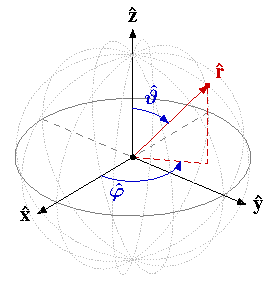
\includegraphics{papers/kugel/figures/tikz/spherical-coordinates}
  \caption{
    Spherical coordinate system. Space is described with the free variables $r
    \in \mathbb{R}_0^+$, $\vartheta \in [0; \pi]$ and $\varphi \in [0; 2\pi)$.
    \label{kugel:fig:spherical-coordinates}
  }
\end{figure}

From Section \ref{buch:pde:section:kugel}, we know that the spherical Laplacian
in the spherical coordinate system (shown in Figure
\ref{kugel:fig:spherical-coordinates}) is is defined as
\begin{equation*}
    \sphlaplacian :=
      \frac{1}{r^2} \frac{\partial}{\partial r} \left(
        r^2 \frac{\partial}{\partial r}
      \right)
      + \frac{1}{r^2} \left[
          \frac{1}{\sin\vartheta} \frac{\partial}{\partial \vartheta} \left(
            \sin\vartheta \frac{\partial}{\partial\vartheta}
          \right)
        + \frac{1}{\sin^2 \vartheta} \frac{\partial^2}{\partial\varphi^2}
      \right].
\end{equation*}
But we will not consider this algebraic monstrosity in its entirety. As the
title suggests, we will only care about the \emph{surface} of the sphere.  This
is for many reasons, but mainly to simplify reduce the already broad scope of
this text. Concretely, we will always work on the unit sphere, which just means
that we set $r = 1$ and keep only $\vartheta$ and $\varphi$ as free variables.
Now, since the variable $r$ became a constant, we can leave out all derivatives
with respect to $r$ and substitute all $r$'s with 1's to obtain a new operator
that deserves its own name.

\begin{definition}[Surface spherical Laplacian]
  \label{kugel:def:surface-laplacian}
  The operator
  \begin{equation*}
      \surflaplacian :=
        \frac{1}{\sin\vartheta} \frac{\partial}{\partial \vartheta} \left(
          \sin\vartheta \frac{\partial}{\partial\vartheta}
        \right)
        + \frac{1}{\sin^2 \vartheta} \frac{\partial^2}{\partial\varphi^2},
  \end{equation*}
  is called the surface spherical Laplacian.
\end{definition}

In the definition, the subscript ``$\partial S$'' was used to emphasize the fact
that we are on the spherical surface, which can be understood as being the
boundary of the sphere. But what does it actually do? To get an intuition, first
of all, notice the fact that $\surflaplacian$ have second derivatives, which
means that this a measure of \emph{curvature}; But curvature of what? To get an
even stronger intuition we will go into geometry, were curvature can be grasped
very well visually. Consider figure \ref{kugel:fig:curvature} where the
curvature is shown using colors: positive curvature in red, and negative
curvature in blue. First we have the curvature of a curve in 1D, then the
curvature of a surface (2D), and finally the curvature of a function on the
surface of the unit sphere.

\begin{figure}
  \centering
  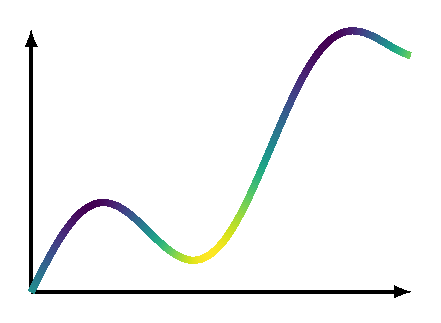
\includegraphics[width=.3\linewidth]{papers/kugel/figures/tikz/curvature-1d}
  \hskip 5mm
  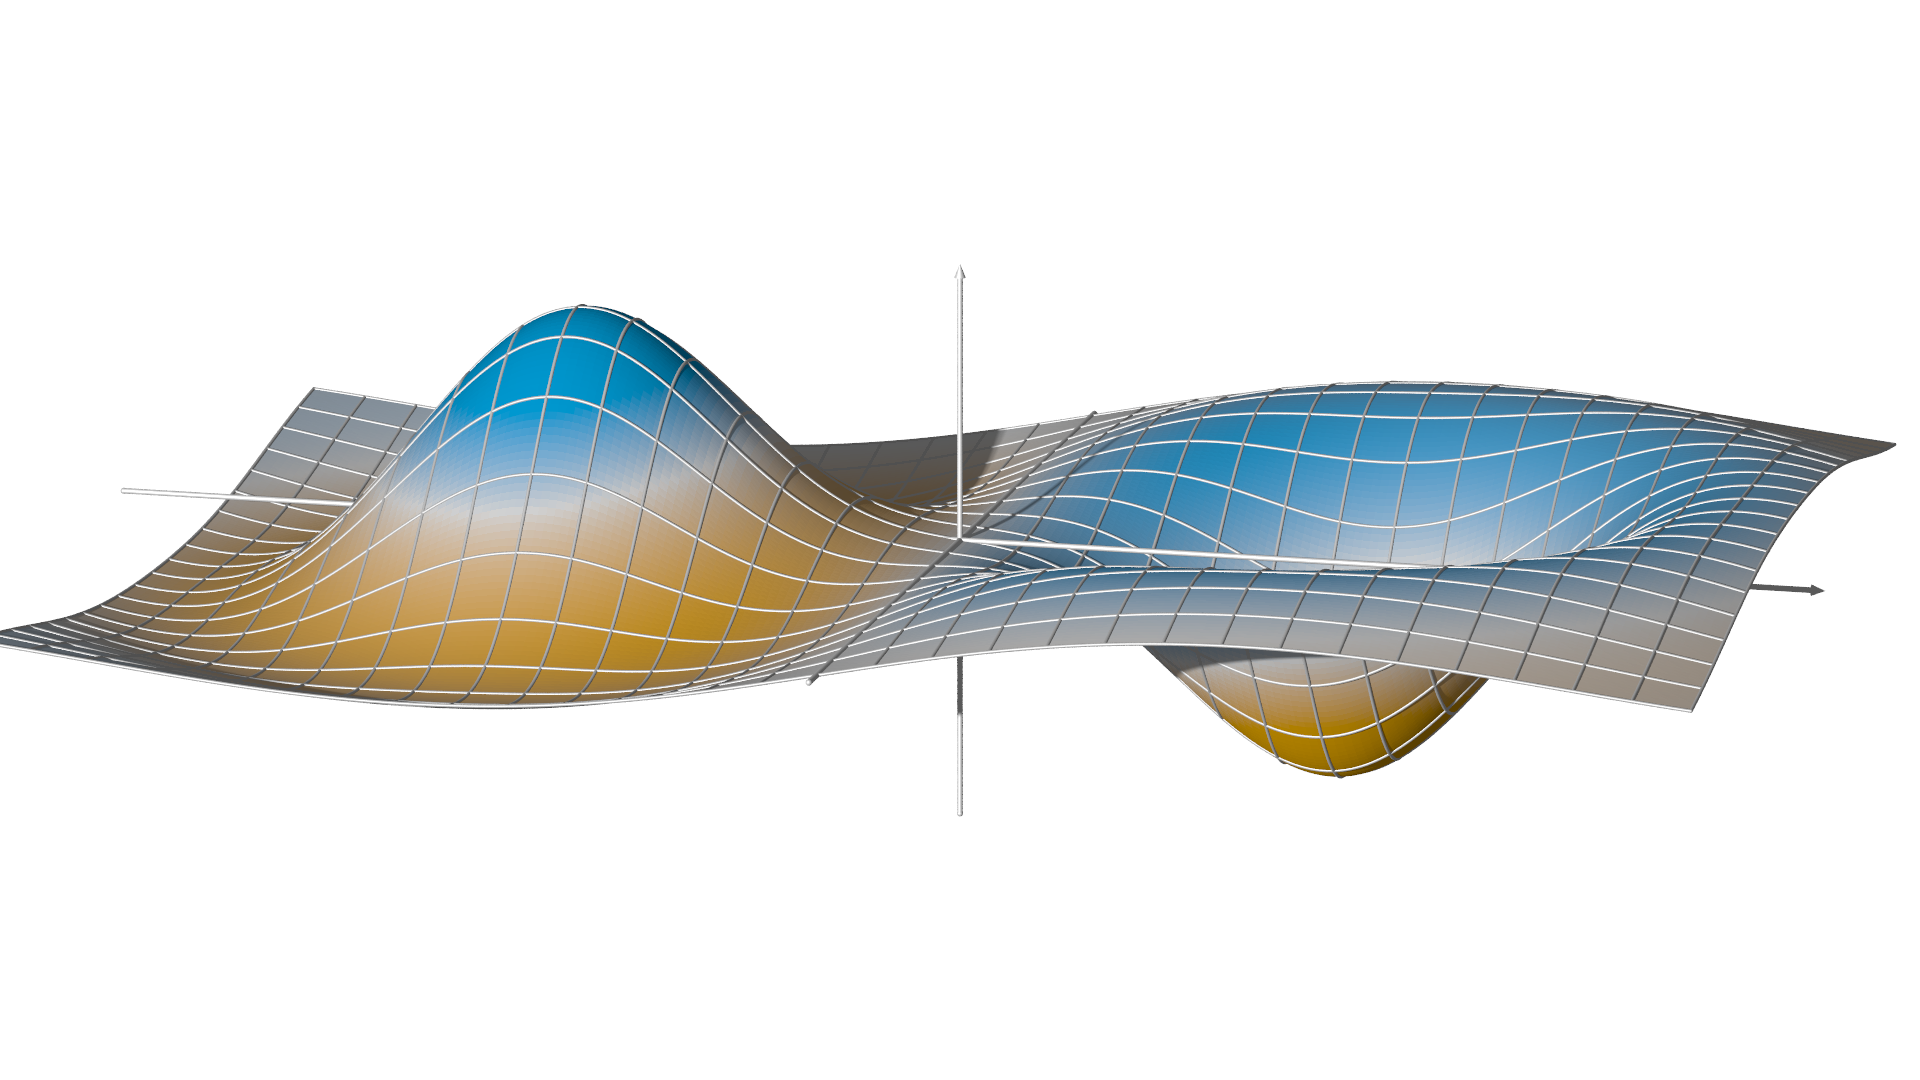
\includegraphics[width=.3\linewidth]{papers/kugel/figures/povray/curvature}
  \hskip 5mm
  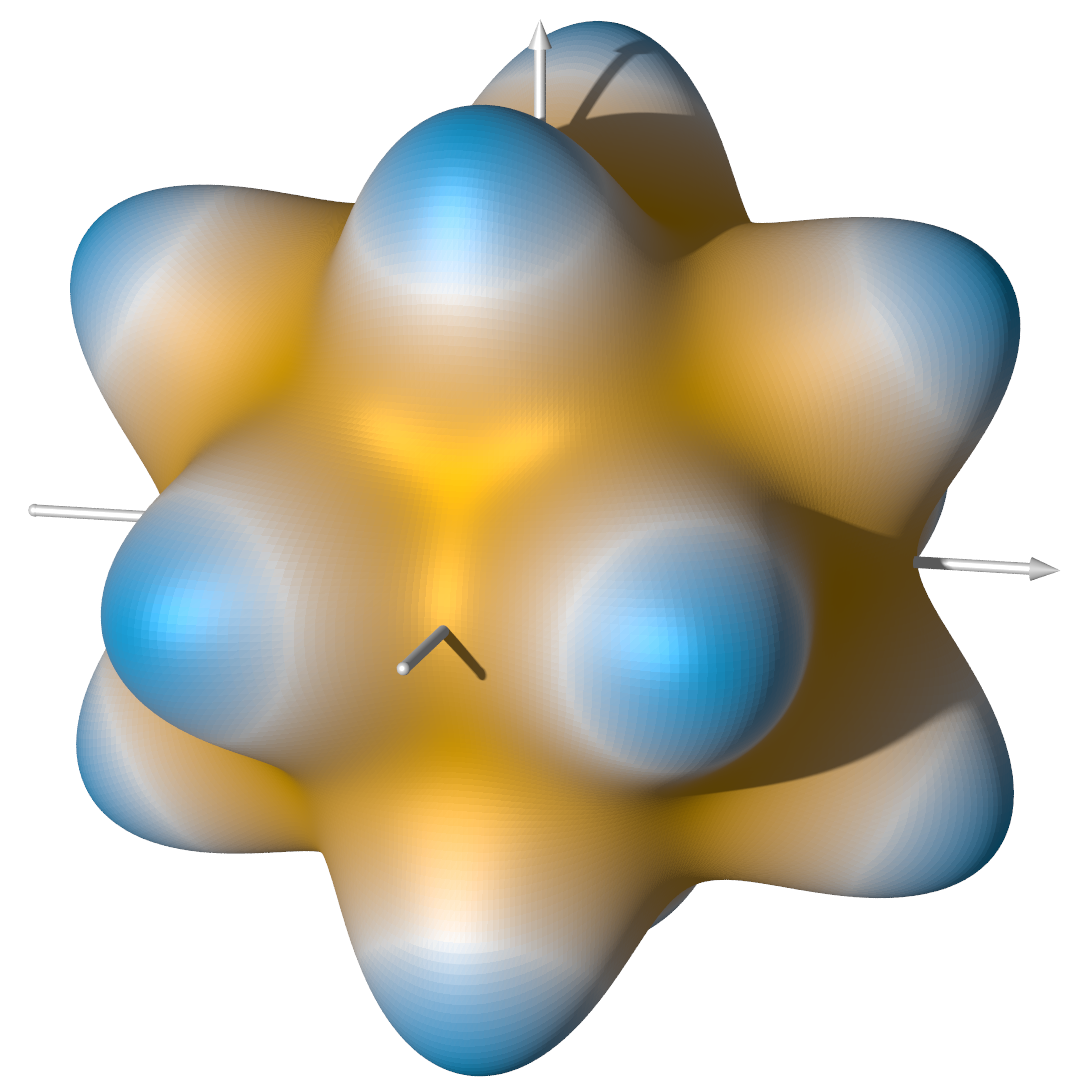
\includegraphics[width=.3\linewidth]{papers/kugel/figures/povray/spherecurve}
  \caption{
    \kugeltodo{Fix alignment / size, add caption. Would be nice to match colors.}
    \label{kugel:fig:curvature}
  }
\end{figure}

Now that we have defined an operator, we can go and study its eigenfunctions,
which means that we would like to find the functions $f(\vartheta, \varphi)$
that satisfy the equation
\begin{equation} \label{kugel:eqn:eigen}
    \surflaplacian f = -\lambda f.
\end{equation}
Perhaps it may not be obvious at first glance, but we are in fact dealing with a
partial differential equation (PDE)\footnote{Considering the fact that we are
dealing with a PDE, you may be wondering what are the boundary conditions. Well,
since this eigenvalue problem is been developed on the spherical surface
(boundary of a sphere), the boundary in this case are empty, i.e no boundary
condition has to be considered.}. If we unpack the notation of the operator
$\nabla^2_{\partial S}$ according to definition
\ref{kugel:def:surface-laplacian}, we get:
\begin{equation} \label{kugel:eqn:eigen-pde}
    \frac{1}{\sin\vartheta} \frac{\partial}{\partial \vartheta} \left(
      \sin\vartheta \frac{\partial f}{\partial\vartheta}
    \right)
    + \frac{1}{\sin^2 \vartheta} \frac{\partial^2 f}{\partial\varphi^2}
    + \lambda f = 0.
\end{equation}
Since all functions satisfying \eqref{kugel:eqn:eigen-pde} are the
\emph{eigenfunctions} of $\surflaplacian$, our new goal is to solve this PDE.
The task may seem very difficult but we can simplify it with a well-known
technique: \emph{the separation Ansatz}. It consists in assuming that the
function $f(\vartheta, \varphi)$ can be factorized in the following form:
\begin{equation}
    f(\vartheta, \varphi) = \Theta(\vartheta)\Phi(\varphi). 
\end{equation}
In other words, we are saying that the effect of the two independent variables
can be described using the multiplication of two functions that describe their
effect separately. This separation process was already presented in section
\ref{buch:pde:section:kugel}, but we will briefly rehearse it here for
convenience. If we substitute this assumption in
\eqref{kugel:eqn:eigen-pde}, we have:
\begin{equation*}
    \frac{1}{\sin\vartheta} \frac{\partial}{\partial \vartheta} \left(
      \sin\vartheta \frac{\partial  \Theta(\vartheta)}{\partial\vartheta}
    \right) \Phi(\varphi)
    + \frac{1}{\sin^2 \vartheta}
      \frac{\partial^2 \Phi(\varphi)}{\partial\varphi^2}
      \Theta(\vartheta)
    + \lambda \Theta(\vartheta)\Phi(\varphi) = 0.
\end{equation*}
Dividing by $\Theta(\vartheta)\Phi(\varphi)$ and introducing an auxiliary
variable $m^2$, the separation constant, yields:
\begin{equation*}
  \frac{1}{\Theta(\vartheta)}\sin \vartheta \frac{d}{d \vartheta} \left(
    \sin \vartheta \frac{d \Theta}{d \vartheta}
  \right)
  + \lambda \sin^2 \vartheta
  = -\frac{1}{\Phi(\varphi)} \frac{d^2\Phi(\varphi)}{d\varphi^2}
  = m^2,
\end{equation*}
which is equivalent to the following system of 2 first order differential
equations (ODEs):
\begin{subequations}
  \begin{gather}
    \frac{d^2\Phi(\varphi)}{d\varphi^2} = -m^2 \Phi(\varphi),
      \label{kugel:eqn:ode-phi} \\ 
    \sin \vartheta \frac{d}{d \vartheta} \left(
      \sin \vartheta \frac{d \Theta}{d \vartheta}
    \right)
    + \left( \lambda - \frac{m^2}{\sin^2 \vartheta} \right)
      \Theta(\vartheta) = 0
      \label{kugel:eqn:ode-theta}.
  \end{gather}
\end{subequations}
The solution of \eqref{kugel:eqn:ode-phi} is easy to find: The complex
exponential is obviously the function we are looking for. So we can directly
write the solutions
\begin{equation} \label{kugel:eqn:ode-phi-sol}
    \Phi(\varphi) = e^{i m \varphi}, \quad m \in \mathbb{Z}.
\end{equation}
The restriction that the separation constant $m$ needs to be an integer arises
from the fact that we require a $2\pi$-periodicity in $\varphi$ since the
coordinate systems requires that $\Phi(\varphi + 2\pi) = \Phi(\varphi)$.
Unfortunately, solving \eqref{kugel:eqn:ode-theta} is not as straightforward,
actually, it is quite difficult, and the process is so involved that it will
require a dedicated section of its own.

\subsection{Legendre Functions}

\begin{figure}
  \centering
  % \kugelplaceholderfig{.8\textwidth}{5cm}
  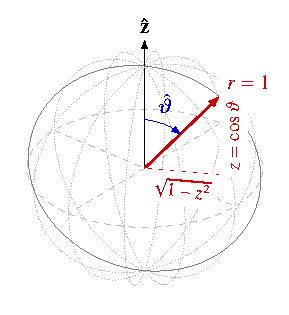
\includegraphics[
    scale = 1.2,
    trim = 0 40 0 0, clip,
  ]{papers/kugel/figures/tikz/legendre-substitution}
  \caption{
    Sketch of the geometry.
    \label{kugel:fig:legendre-substitution}
  }
\end{figure}

To solve \eqref{kugel:eqn:ode-theta} we start with the substitution $z = \cos
\vartheta$, which has a neat geometrical justification. To see it consider
figure \ref{kugel:fig:legendre-substitution}, where we sketched the geometry of
the problem. Algebraically, the operator $\frac{d}{d \vartheta}$ becomes
\begin{equation*}
    \frac{d}{d \vartheta}
    = \frac{dz}{d \vartheta}\frac{d}{dz}
    = -\sin \vartheta \frac{d}{dz}
    = -\sqrt{1-z^2} \frac{d}{dz},
\end{equation*} 
since $\sin \vartheta = \sqrt{1 - \cos^2 \vartheta} = \sqrt{1 - z^2}$, which
agrees with our sketch. Thus, \eqref{kugel:eqn:ode-theta} becomes 
\begin{align*}
  \frac{-\sqrt{1-z^2}}{\sqrt{1-z^2}} \frac{d}{dz} \left[
    \left(\sqrt{1-z^2}\right) \left(-\sqrt{1-z^2}\right) \frac{d \Theta}{dz}
  \right]
  + \left( \lambda - \frac{m^2}{1 - z^2} \right)\Theta(\vartheta) &= 0,
  \\
  \frac{d}{dz} \left[ (1-z^2) \frac{d \Theta}{dz} \right]
  + \left( \lambda - \frac{m^2}{1 - z^2} \right)\Theta(\vartheta) &= 0,
  \\
  (1-z^2)\frac{d^2 \Theta}{dz} - 2z\frac{d \Theta}{dz}
  + \left( \lambda - \frac{m^2}{1 - z^2} \right)\Theta(\vartheta) &= 0.
\end{align*}
By making two final cosmetic substitutions, namely $Z(z) = \Theta(\cos^{-1}z)$
and $\lambda = n(n+1)$, we obtain what is known in the literature as the
\emph{associated Legendre equation of order $m$}:
\nocite{olver_introduction_2013}
\begin{equation} \label{kugel:eqn:associated-legendre}
  (1 - z^2)\frac{d^2 Z}{dz^2}
  - 2z\frac{d Z}{dz}
  + \left( n(n + 1) - \frac{m^2}{1 - z^2} \right) Z(z) = 0,
  \quad
  z \in [-1; 1], m \in \mathbb{Z}.
\end{equation}

Our new goal has therefore become to solve
\eqref{kugel:eqn:associated-legendre}, since if we find a solution for $Z(z)$ we
can perform the substitution backwards and get back to our eigenvalue problem.
However, the associated Legendre equation is not any easier, so to attack the
problem we will look for the solutions in the easier special case when $m = 0$.
This reduces the problem because it removes the double pole, which is always
tricky to deal with. In fact, the reduced problem when $m = 0$ is known as the
\emph{Legendre equation}:
\begin{equation} \label{kugel:eqn:legendre}
  (1 - z^2)\frac{d^2 Z}{dz^2}
  - 2z\frac{d Z}{dz}
  + n(n + 1) Z(z) = 0,
  \quad
  z \in [-1; 1].
\end{equation}

The Legendre equation is a second order differential equation, and therefore it
has 2 independent solutions, which are known as \emph{Legendre functions} of the
first and second kind. For the scope of this text we will only derive a special
case of the former that is known known as the \emph{Legendre polynomials}, since
we only need a solution between $-1$ and $1$.

\begin{lemma}[Legendre polynomials]
  \label{kugel:thm:legendre-poly}
  The polynomial function
  \[
    P_n(z) = \sum^{\lfloor n/2 \rfloor}_{k=0}
      \frac{(-1)^k}{2^n s^k!} \frac{(2n - 2k)!}{(n - k)! (n-2k)!} z^{n - 2k}
  \]
  is the only finite solution of the Legendre equation
  \eqref{kugel:eqn:legendre} when $n \in \mathbb{Z}$ and $z \in [-1; 1]$.
\end{lemma}
\begin{proof}
  This results is derived in section \ref{kugel:sec:proofs:legendre}.
\end{proof}

Since the Legendre \emph{polynomials} are indeed polynomials, they can also be
expressed using the hypergeometric functions described in section
\ref{buch:rekursion:section:hypergeometrische-funktion}, so in fact
\begin{equation}
  P_n(z) = {}_2F_1 \left( \begin{matrix}
    n + 1, & -n \\ \multicolumn{2}{c}{1}
  \end{matrix} ; \frac{1 - z}{2} \right).
\end{equation}
Further, there are a few more interesting but not very relevant forms to write
$P_n(z)$ such as \emph{Rodrigues' formula} and \emph{Laplace's integral
representation} which are
\begin{equation*}
  P_n(z) = \frac{1}{2^n n!} \frac{d^n}{dz^n} (z^2 - 1)^n,
  \qquad \text{and} \qquad
  P_n(z) = \frac{1}{\pi} \int_0^\pi \left(
    z + \cos\vartheta \sqrt{z^2 - 1}
  \right) \, d\vartheta
\end{equation*}
respectively, both of which we will not prove (see chapter 3 of
\cite{bell_special_2004} for a proof). Now that we have a solution for the
Legendre equation, we can make use of the following lemma to patch the solutions
such that they also become solutions of the associated Legendre equation
\eqref{kugel:eqn:associated-legendre}.

\begin{lemma} \label{kugel:thm:extend-legendre}
  If $Z_n(z)$ is a solution of the Legendre equation \eqref{kugel:eqn:legendre},
  then
  \begin{equation*}
    Z^m_n(z) = (1 - z^2)^{m/2} \frac{d^m}{dz^m}Z_n(z)
  \end{equation*}
  solves the associated Legendre equation \eqref{kugel:eqn:associated-legendre}.
  \nocite{bell_special_2004}
\end{lemma}
\begin{proof}
  See section \ref{kugel:sec:proofs:legendre}.
\end{proof}

What is happening in lemma \ref{kugel:thm:extend-legendre}, is that we are
essentially inserting a square root function in the solution in order to be able
to reach the parts of the domain near the poles at $\pm 1$ of the associated
Legendre equation, which is not possible only using power series
\kugeltodo{Reference book theory on extended power series method.}. Now, since
we have a solution in our domain, namely $P_n(z)$, we can insert it in the lemma 
obtain the \emph{associated Legendre functions}.

\begin{definition}[Ferrers or associated Legendre functions]
  \label{kugel:def:ferrers-functions}
  The functions
  \begin{equation}
    P^m_n (z) = (1-z^2)^{\frac{m}{2}}\frac{d^{m}}{dz^{m}} P_n(z)
      = \frac{1}{2^n n!}(1-z^2)^{\frac{m}{2}}\frac{d^{m+n}}{dz^{m+n}}(1-z^2)^n, \quad |m|<n
  \end{equation}
  are known as Ferrers or associated Legendre functions.
\end{definition}
The constraint $|m|<n$, can be justified by considering eq.\eqref{kugel:eq:associated_leg_func}, where we differentiate $m+n$ times. We all know that a differentiation, to be well defined, must have an order that is greater than zero \kugeltodo{is that always true?}. Furthermore, it can be seen that this derivative is applied on a polynomial of degree $2n$. As is known from Calculus 1, if you derive a polynomial of degree $2n$ more than $2n$ times, you get zero, that would be a trivial solution. This is the power of zero: It is almost always a (boring) solution.

We can thus summarize these two conditions by writing:
\begin{equation*}
    \begin{rcases}
        m+n \leq 2n &\implies m \leq n \\
        m+n \geq 0  &\implies  m \geq -n
    \end{rcases} \; |m| \leq n.
\end{equation*}

\subsection{Spherical Harmonics}

Finally, we can go back to solving our boundary value problem we started in
section \ref{kugel:sec:construction:eigenvalue}. We had left off in the middle
of the separation, were we had used the Ansatz $f(\vartheta, \varphi) =
\Theta(\vartheta) \Phi(\varphi)$ to find that $\Phi(\varphi) = e^{im\varphi}$,
and we were solving for $\Theta(\vartheta)$.  As you may recall, previously we
performed the substitution $z = \cos \vartheta$. Now we can finally bring back the
solution to the associated Legendre equation $P^m_n(z)$ into the $\vartheta$
domain and combine it with $\Phi(\varphi)$ to get the full result:
\begin{equation*}
    f(\vartheta, \varphi)
      = \Theta(\vartheta)\Phi(\varphi)
      = P^m_n (\cos \vartheta) e^{im\varphi}, \quad |m|<n.
\end{equation*}
This family of functions, which recall are the solutions of the eigenvalue
problem of the surface spherical Laplacian, are the long anticipated
\emph{complex spherical harmonics}, and they are usually denoted with
$Y^m_n(\vartheta, \varphi)$.

\begin{definition}[Spherical harmonics]
  \label{kugel:def:spherical-harmonics}
  The functions
  \begin{equation*}
    Y^m_n (\vartheta, \varphi) = P^m_n(\cos \vartheta) e^{im\varphi}, \quad |m|<n
  \end{equation*}
  where $m, n \in \mathbb{Z}$ are called (unnormalized) spherical
  harmonics.
\end{definition}

\begin{figure}
  \centering
  \kugelplaceholderfig{\textwidth}{.8\paperheight}
  \caption{
    \kugeltodo{Big picture with the first few spherical harmonics.}
    \label{kugel:fig:spherical-harmonics}
  }
\end{figure}

\kugeltodo{Describe how they look like with fig.
\ref{kugel:fig:spherical-harmonics}}

\subsection{Orthogonality of $P_n$, $P^m_n$ and $Y^m_n$}

We shall now discuss an important property of the spherical harmonics: they form
an orthogonal system. And since the spherical harmonics contain the Ferrers or
associated Legendre functions, we need to discuss their orthogonality first.
But the Ferrers functions themselves depend on the Legendre polynomials, so that
will be our starting point.

\begin{lemma} For the Legendre polynomials $P_n(z)$ and $P_k(z)$ it holds that
  \label{kugel:thm:legendre-poly-ortho}
  \begin{equation*}
    \int_{-1}^1 P_n(z) P_k(z) \, dz
    = \frac{2}{2n + 1} \delta_{nk}
    = \begin{cases}
      \frac{2}{2n + 1} & \text{if } n = k, \\
      0 & \text{otherwise}.
    \end{cases}
  \end{equation*}
\end{lemma}
\begin{proof}
  To start, consider the fact that the Legendre equation
  \eqref{kugel:eqn:legendre}, of which two distinct Legendre polynomials
  $P_n(z)$ and $P_k(z)$ are a solution ($n \neq k$), can be rewritten in the
  following form:
  \begin{equation}
    \frac{d}{dz} \left[ 
      \left( 1 - z^2 \right) \frac{dZ}{dz}
    \right] + n(n+1) Z(z) = 0.
  \end{equation}
  So we rewrite the Legendre equations for $P_n(z)$ and $P_k(z)$:
  \begin{align*}
    \frac{d}{dz} \left[ 
      \left( 1 - z^2 \right) \frac{dP_n}{dz}
    \right] + n(n+1) P_n(z) &= 0,
    &
    \frac{d}{dz} \left[ 
      \left( 1 - z^2 \right) \frac{dP_k}{dz}
    \right] + k(k+1) P_k(z) &= 0,
  \end{align*}
  then we multiply the former by $P_k(z)$ and the latter by $P_n(z)$ and
  subtract the two to get
  \begin{equation*}
    \frac{d}{dz} \left[ 
      \left( 1 - z^2 \right) \frac{dP_n}{dz}
    \right] P_k(z) + n(n+1) P_n(z) P_k(z)
    -
    \frac{d}{dz} \left[ 
      \left( 1 - z^2 \right) \frac{dP_k}{dz}
    \right] P_n(z) - k(k+1) P_k(z) P_n(z) = 0.
  \end{equation*}
  By grouping terms, making order and integrating with respect to $z$ from $-1$
  to 1 we obtain
  \begin{gather}
    \int_{-1}^1 \left\{
      \frac{d}{dz} \left[ 
        \left( 1 - z^2 \right) \frac{dP_n}{dz}
      \right] P_k(z) 
      -
      \frac{d}{dz} \left[ 
        \left( 1 - z^2 \right) \frac{dP_k}{dz}
      \right] P_n(z) - k(k+1) P_k(z) P_n(z)
    \right\} \,dz \nonumber \\
    + \left[ n(n+1) - k(k+1) \right] \int_{-1}^1 P_k(z) P_n(z) \, dz = 0.
    \label{kugel:thm:legendre-poly-ortho:proof:1}
  \end{gather}
  Since by the product rule
  \begin{equation*}
    \frac{d}{dz} \left[ (1 - z^2) \frac{dP_k}{dz} P_n(z) \right]
    =
    \frac{d}{dz} \left[ (1 - z^2) \frac{dP_n}{dz} \right] P_k(z)
      + (1 - z^2) \frac{dP_n}{dz} \frac{dP_k}{dz},
  \end{equation*}
  we can simplify the first term in
  \eqref{kugel:thm:legendre-poly-ortho:proof:1} to get
  \begin{gather*}
    \int_{-1}^1 \left\{
      \frac{d}{dz} \left[ (1 - z^2) \frac{dP_k}{dz} P_n(z) \right]
        - \cancel{(1 - z^2) \frac{dP_n}{dz} \frac{dP_k}{dz}}
        - \frac{d}{dz} \left[ (1 - z^2) \frac{dP_n}{dz} P_k(z) \right]
        + \cancel{(1 - z^2) \frac{dP_k}{dz} \frac{dP_n}{dz}}
    \right\} \, dz \\
    = \int_{-1}^1 \frac{d}{dz} \left\{ (1 - z^2) \left[
      \frac{dP_k}{dz} P_n(z) - \frac{dP_n}{dz} P_k(z)
    \right] \right\} \, dz
    = (1 - z^2) \left[
      \frac{dP_k}{dz} P_n(z) - \frac{dP_n}{dz} P_k(z)
    \right] \Bigg|_{-1}^1,
  \end{gather*}
  which always equals 0 because the product contains $1 - z^2$ and the bounds
  are at $\pm 1$. Thus, of \eqref{kugel:thm:legendre-poly-ortho:proof:1} only
  the second term remains and the equation becomes
  \begin{equation*}
    \left[ n(n+1) - k(k+1) \right] \int_{-1}^1 P_k(z) P_n(z) \, dz = 0.
  \end{equation*}
  By dividing by the constant in front of the integral we have our first result.
  Now we need to show that when $n = k$ the integral equals $2 / (2n + 1)$.
  % \begin{equation*}
  % \end{equation*}
  \kugeltodo{Finish proof. Can we do it without the generating function of
  $P_n$?}
\end{proof}

In a similarly algebraically tedious fashion, we can also continue to check for
orthogonality for the Ferrers functions $P^m_n(z)$, since they are related to
$P_n(z)$ by a $m$-th derivative, and obtain the following result.

\begin{lemma} For the associated Legendre functions
  \label{kugel:thm:associated-legendre-ortho}
  \begin{equation*}
    \int_{-1}^1 P^m_n(z) P^{m}_{n'}(z) \, dz
    = \frac{2(m + n)!}{(2n + 1)(n - m)!} \delta_{nn'}
    = \begin{cases}
      \frac{2(m + n)!}{(2n + 1)(n - m)!}
        & \text{if } n = n', \\
      0 & \text{otherwise}.
    \end{cases}
  \end{equation*}
\end{lemma}
\begin{proof}
  To show that the expression equals zero when $n \neq n'$ we can perform
  exactly the same steps as in the proof of lemma
  \ref{kugel:thm:legendre-poly-ortho}, so we will not repeat them here and prove
  instead only the case when $n = n'$.
  \kugeltodo{Finish proof, or not? I have to look and decide if it is
  interesting enough.}
\end{proof}

By having the orthogonality relations of the Legendre functions we can finally
show that spherical harmonics are also orthogonal under the following inner
product:

\begin{definition}[Inner product in $S^2$]
  \label{kugel:def:inner-product-s2}
  For two complex valued functions $f(\vartheta, \varphi)$ and $g(\vartheta,
  \varphi)$ on the surface of the sphere the inner product is defined to be
  \begin{equation*}
    \langle f, g \rangle
    = \int_{0}^\pi \int_0^{2\pi}
      f(\vartheta, \varphi) \overline{g(\vartheta, \varphi)}
      \sin \vartheta \, d\varphi \, d\vartheta.
  \end{equation*}
\end{definition}


\begin{theorem} For the (unnormalized) spherical harmonics
  \label{kugel:thm:spherical-harmonics-ortho}
  \begin{align}
    \langle Y^m_n, Y^{m'}_{n'} \rangle
    &= \int_{0}^\pi \int_0^{2\pi}
      Y^m_n(\vartheta, \varphi) \overline{Y^{m'}_{n'}(\vartheta, \varphi)}
      \sin \vartheta \, d\varphi \, d\vartheta
      \label{kugel:eq:spherical-harmonics-inner-prod} \\
    &= \frac{4\pi}{2n + 1} \frac{(m + n)!}{(n - m)!} \delta_{nn'} \delta_{mm'}
    = \begin{cases}
      \frac{4\pi}{2n + 1} \frac{(m + n)!}{(n - m)!}
        & \text{if } n = n' \text{ and } m = m', \nonumber \\
      0 & \text{otherwise}.
    \end{cases}
  \end{align}
\end{theorem}
\begin{proof}
  We will begin by doing a bit of algebraic maipulaiton:
  \begin{align*}
    \int_{0}^\pi \int_0^{2\pi}
      Y^m_n(\vartheta, \varphi) \overline{Y^{m'}_{n'}(\vartheta, \varphi)} 
      \sin \vartheta \, d\varphi \, d\vartheta
    &= \int_{0}^\pi \int_0^{2\pi}
      e^{im\varphi} P^m_n(\cos \vartheta)
      e^{-im'\varphi} P^{m'}_{n'}(\cos \vartheta)
      \, d\varphi \sin \vartheta \, d\vartheta 
    \\
    &= \int_{0}^\pi
      P^m_n(\cos \vartheta) P^{m'}_{n'}(\cos \vartheta) \sin \vartheta \, d\vartheta
      \int_0^{2\pi} e^{i(m - m')\varphi}
      \, d\varphi. 
  \end{align*}
  First, notice that the associated Legendre polynomials are assumed to be real,
  and are thus unaffected by the complex conjugation. Then, we can see that when
  $m = m'$ the inner integral simplifies to $\int_0^{2\pi} 1 \, d\varphi$ which
  equals $2\pi$, so in this case the expression becomes
  \begin{equation*}
    2\pi \int_{0}^\pi
      P^m_n(\cos \vartheta) P^{m'}_{n'}(\cos \vartheta)
    \sin \vartheta \, d\vartheta
    = -2\pi \int_{1}^{-1} P^m_n(z) P^{m'}_{n'}(z) \, dz
    = \frac{4\pi(m + n)!}{(2n + 1)(n - m)!} \delta_{nn'},
  \end{equation*}
  where in the second step we performed the substitution $z = \cos\vartheta$;
  $d\vartheta = \frac{d\vartheta}{dz} dz= - dz / \sin \vartheta$, and then we
  used lemma \ref{kugel:thm:associated-legendre-ortho}. 
  We are allowed to use
  the lemma because $m = m'$. After the just mentioned substitution we can write eq.\eqref{kugel:eq:spherical-harmonics-inner-prod} in this form
  \begin{equation*}
    \langle Y^m_n, Y^{m'}_{n'} \rangle_{\partial S} = \langle P^m_n, P^{m'}_{n'} \rangle_z \; \langle e^{im\varphi}, e^{-im'\varphi} \rangle_\varphi.
  \end{equation*} 
  Now we just need look at the case when $m \neq m'$. Fortunately this is
  easier: the inner integral is $\int_0^{2\pi} e^{i(m - m')\varphi} d\varphi$,
  or in other words we are integrating a complex exponential over the entire
  period, which always results in zero. Thus, we do not need to do anything and
  the proof is complete.
\end{proof}

These proofs for the various orthogonality relations were quite long and
algebraically tedious, mainly because they are ``low level'', by which we mean
that they (arguably) do not rely on very abstract theory. However, if we allow
ourselves to use the more abstract Sturm Liouville theory discussed in chapters
\ref{buch:integrale:subsection:sturm-liouville-problem} and \kugeltodo{reference
to chapter 17 of haddouche and Löffler} the proofs can become ridiculously
short. Let's do for example lemma \ref{kugel:thm:associated-legendre-ortho}.

\begin{proof}[
    Shorter proof of lemma \ref{kugel:thm:associated-legendre-ortho}
  ]
  The associated Legendre polynomials, of which we would like to prove an
  orthogonality relation, are the solution to the associated Legendre equation,
  which we can write as $LZ(z) = 0$, where
  \begin{equation*}
    L = \frac{d}{dz} (1 - z^2) \frac{d}{dz}
      + n(n+1) - \frac{m^2}{1 - z^2}.
  \end{equation*}
  Notice that $L$ is in fact a Sturm-Liouville operator of the form
  \begin{equation*}
    L = \frac{1}{w(z)} \left[
        \frac{d}{dz} p(z) \frac{d}{dz} - \lambda + q(z)
      \right],
  \end{equation*}
  if we let $w(z) = 1$, $p(z) = (1 - z^2 )$, $q(z) = -m^2 / (1 - z^2)$, and
  $\lambda = -n(n+1)$. By the theory of Sturm-Liouville operators, we know that
  the each solution of the problem $LZ(z) = 0$, namely $P^m_n(z)$, is orthogonal
  to every other solution that has a different $\lambda$. In our case $\lambda$
  varies with $n$, so $P^m_n(z)$ with different $n$'s are orthogonal to each
  other.
\end{proof}

But that was still rather informative and had a bit of explanation, which is
terrible. Real snobs, such as Wikipedia contributors, some authors and
regrettably sometimes even ourselves, would write instead:

\begin{proof}[
    Infuriatingly short proof of lemma \ref{kugel:thm:associated-legendre-ortho}
  ]
  The associated Legendre polynomials are solutions of the associated Legendre
  equation which is a Sturm-Liouville problem and are thus orthogonal to each
  other. The factor in front Kronecker delta is left as an exercise to the
  reader.
\end{proof}

Lemma \ref{kugel:thm:legendre-poly-ortho} has a very similar proof, while the
theorem \ref{kugel:thm:spherical-harmonics-ortho} for the spherical harmonics is
proved by the following argument.  The spherical harmonics are the solutions to
the eigenvalue problem $\surflaplacian f = -\lambda f$, which as discussed in
the previous section is solved using the separation Ansatz. So to prove their
orthogonality using the Sturm-Liouville theory we argue that
\begin{equation*}
  \surflaplacian = L_\vartheta L_\varphi \iff
  \surflaplacian f(\vartheta, \varphi)
    = L_\vartheta \Theta(\vartheta) L_\varphi \Phi(\varphi),
\end{equation*}
then we show that both $L_\vartheta$ and $L_\varphi$ are both Sturm-Liouville
operators (we just did the former in the shorter proof above). Since both are
Sturm-Liouville operators their combination, the surface spherical Laplacian, is
also a Sturm-Liouville operator, which then implies orthogonality.

\subsection{Normalization and the Phase Factor}

At this point we have shown that the spherical harmonics form an orthogonal
system, but in many applications we usually also want a normalization of some
kind. For example the most obvious desirable property could be for the spherical
harmonics to be ortho\emph{normal}, by which we mean that $\langle Y^m_n,
Y^{m'}_{n'} \rangle = \delta_{nn'}$. To obtain orthonormality, we simply add an
ugly normalization factor in front of the previous definition
\ref{kugel:def:spherical-harmonics} as follows.

\begin{definition}[Orthonormal spherical harmonics]
  \label{kugel:def:spherical-harmonics-orthonormal}
  The functions
  \begin{equation*}
    Y^m_n(\vartheta, \varphi)
    = \sqrt{\frac{2n + 1}{4\pi} \frac{(n-m)!}{(m+n)!}}
      P^m_n(\cos \vartheta) e^{im\varphi}
  \end{equation*}
  where $m, n \in \mathbb{Z}$ and $|m| < n$ are the orthonormal spherical
  harmonics.
\end{definition}

Orthornomality is very useful, but it is not the only common normalization that
is found in the literature. In physics, geomagnetism to be more specific, it is
common to use the so called Schmidt semi-normalization (or sometimes also called
quasi-normalization).

\begin{definition}[Schmidt semi-normalized spherical harmonics]
  \label{kugel:def:spherical-harmonics-schmidt}
  The Schmidt semi-normalized spherical harmonics are
  \begin{equation*}
    Y^m_n(\vartheta, \varphi)
    = \sqrt{2 \frac{(n - m)!}{(n + m)!}}
      P^m_n(\cos \vartheta) e^{im\varphi}
  \end{equation*}
  where $m, n \in \mathbb{Z}$ and $|m| < n$.
\end{definition}

Additionally, there is another quirk in the literature that should be mentioned.
In some other branches of physics such as seismology and quantum mechanics there
is a so called Condon-Shortley phase factor $(-1)^m$ in front of the square root
in the definition of the normalized spherical harmonics. It is yet another
normalization that is added for physical reasons that are not very relevant to
our discussion, but we mention this potential source of confusion since many
numerical packages (such as \texttt{SHTOOLS}
\cite{markwieczorek_shtoolsshtools_2022}) offer an option to add or remove it
from the computation.

Though, for our purposes we will mostly only need the orthonormal spherical
harmonics, so from now on, unless specified otherwise when we say spherical
harmonics or write $Y^m_n$, we mean the orthonormal spherical harmonics of
definition \ref{kugel:def:spherical-harmonics-orthonormal}.

\subsection{Recurrence Relations}\kugeltodo{replace x with z}
The idea of this subsection is to introduce first some recursive relations regarding the Associated Legendre Functions, defined in eq.\eqref{kugel:def:ferrers-functions}. Subsequently we will extend them, in order to derive recurrence formulas for the case of Spherical Harmonic functions as well. 
\subsubsection{Associated Legendre Functions}
To start this journey, we can first write the following equations, which relate the Associated Legendre functions of different indeces $m$ and $n$ recursively:
\begin{subequations}
  \begin{align}
  P^m_n(z) &= \dfrac{1}{(2n+1)x} \left[ (m+n) P^m_{n-1}(z) + (n-m+1) P^m_{n+1}(z) \right] \label{kugel:eq:rec-leg-1} \\
  P^m_n(z) &= \dfrac{\sqrt{1-z^2}}{2mz} \left[ P^{m+1}_n(z) + [n(n+1)-m(m-1)] P^{m-1}_n(z) \right] \label{kugel:eq:rec-leg-2} \\ 
  P^m_n(z) &= \dfrac{1}{(2n+1)\sqrt{1-z^2}} \left[ P^{m+1}_{n+1}(z) - P^{m+1}_{n-1}(z) \right]  \label{kugel:eq:rec-leg-3} \\
  P^m_n(z) &= \dfrac{1}{(2n+1)\sqrt{1-z^2}} \left[ (n+m)(n+m-1)P^{m-1}_{n-1}(z) - (n-m+1)(n-m+2)P^{m-1}_{n+1}(z) \right]  \label{kugel:eq:rec-leg-4}
  \end{align}
\end{subequations}
Much of the effort will be proving this bunch of equalities. Then, in the second part, where we will derive the recursion equations for $Y^m_n(\vartheta,\varphi)$, we will basically reuse the ones presented above.

Maybe it is worth mentioning at least one use case for these relations: In some software implementations (that include lighting computations in computer graphics, antenna modelling softwares, 3-D modelling in medical applications, etc.) 
they are widely used, as they lead to better numerical accuracy and computational cost lower by a factor of six\cite{usecase_recursion_paper}. 
\begin{enumerate}[(i)]
  \item 
  \begin{proof}
    This is the relation that links the associated Legendre functions with the same $m$ index but different $n$. Using \ref{} \kugeltodo{search the general equation of recursion for orthogonal polynomials (is somewhere in the book)}, we have 
    \begin{equation*}
      (n+1)P_{n+1}(z)-(2n+1)xP_n(z)+nP_{n-1}(z)=0,
    \end{equation*}
    that can be differentiated $m$ times, obtaining
    \begin{equation}\label{kugel:eq:rec_1}
      (n+1)\frac{d^mP_{n+1}}{dz^m}-(2n+1) \left[z \frac{d^m P_n}{dz^m}+ m\frac{d^{m-1}P_{n-1}}{dz^{m-1}} \right] + n\frac{d^m P_{n-1}}{dz^m}=0.
    \end{equation}
    To continue this derivation, we need the following relation:
    \begin{equation}\label{kugel:eq:rec_2}
      \frac{dP_{n+1}}{dz} - \frac{dP_{n-1}}{dz} = (2n+1)P_n.
    \end{equation}
    The latter will not be derived, because it suffices to use the definition of the Legendre Polynomials $P_n(x)$ to check it.
    
    We can now differentiate the just presented eq.\eqref{kugel:eq:rec_2} $m-1$ times, that will become
    \begin{equation}\label{kugel:eq:rec_3}
      \frac{d^mP_{n+1}}{dx^m} - \frac{d^mP_{n-1}}{dx^m} = (2n+1)\frac{d^{m-1}P_n}{dx^{m-1}}.
    \end{equation}
    Then, using eq.\eqref{kugel:eq:rec_3} in eq.\eqref{kugel:eq:rec_1}, we will have
    \begin{equation}\label{kugel:eq:rec_4}
      (n+1)\frac{d^mP_{n+1}}{dx^m}- (2n+1)\frac{d^mP_{n+1}}{dx^m} -m\left[\frac{d^m P_{n+1}}{dx^m}+ \frac{d^{m}P_{n-1}}{dx^m}\right] + n\frac{d^m P_{n-1}}{dx^m}=0.
    \end{equation}
    Finally, multiplying both sides by $(1-x^2)^{\frac{m}{2}}$ and simplifying the expression, we can rewrite eq.\eqref{kugel:eq:rec_4} in terms of $P^m_n(x)$, namely
    \begin{equation*}
      (n+1-m)P^m_{n+1}(x)-(2n+1)xP^m_n(x)+(m+n)P^m_{n-1}(x)=0,
    \end{equation*}
    that rearranged, will be
    \begin{equation*}
      (2n+1) x P^m_n(x)= (m+n) P^m_{n-1}(x) + (n-m+1) P^m_{n+1}(x).
    \end{equation*}
  \end{proof}
  
  \item
  \begin{proof}
    This relation, unlike the previous one, link three expression with the same $n$ index but different $m$. 
    
    In the proof of Lemma \ref{kugel:lemma:sol_associated_leg_eq}, at some point we ran into this expression.
    \begin{equation*}
      (1-x^2)\frac{d^{m+2}P_n}{dx^{m+2}} - 2(m+1)x \frac{d^{m+1}P_n}{dx^{m+1}} + [n(n+1)-m(m+1)]\frac{d^mP_n}{dx^m} = 0,
    \end{equation*}
    that, if multiplied by $(1-x^2)^{\frac{m}{2}}$, will be
    \begin{equation*}
      (1-x^2)^{\frac{m}{2}+1}\frac{d^{m+2}P_n}{dx^{m+2}} - 2(m+1)x (1-x^2)^{\frac{m}{2}}\frac{d^{m+1}P_n}{dx^{m+1}} + [n(n+1)-m(m+1)](1-x^2)^{\frac{m}{2}}\frac{d^mP_n}{dx^m} = 0.
    \end{equation*}
    Therefore, as before, expressing it in terms of $P^m_n(x)$:
    \begin{equation*}
      P^{m+2}_n(x) - \frac{2(m+1)x}{\sqrt{1-x^2}}P^{m+1}_n(x) + [n(n+1)-m(m+1)]P^m_n(x)=0.
    \end{equation*}
    Further, we can adjust the indeces and terms, obtaining
    \begin{equation*}
      \frac{2mx}{\sqrt{(1-x^2)}} P^m_n(x) = P^{m+1}_n(x) + [n(n+1)-m(m-1)] P^{m-1}_n(x).
    \end{equation*}
  
  \end{proof}
  
  \item
  \begin{proof}
    To derive this expression, we can multiply eq.\eqref{kugel:eq:rec_3} by $(1-x^2)^{\frac{m}{2}}$ and, as always, we could express it in terms of $P^m_n(x)$:
    \begin{equation*}
      P^m_{n+1}(x) - P^m_{n-1}(x) = (2n+1)\sqrt{1-x^2}P^{m-1}_n(x).
    \end{equation*}
    Afer that we can divide by $2n+1$ resulting in
    \begin{equation}\label{kugel:eq:helper}
      \frac{1}{2n+1}[P^m_{n+1}(x) - P^m_{n-1}(x)] = \sqrt{1-x^2}P^{m-1}_n(x).
    \end{equation}
    To conclude, we arrange the indeces differently:
    \begin{equation*}
      \sqrt{1-x^2}P^{m}_n(x)=\frac{1}{2n+1}[P^{m+1}_{n+1}(x) - P^{m+1}_{n-1}(x)].
    \end{equation*}
  \end{proof}

  \item
  \begin{proof}
    For this proof we can rely on eq.\eqref{kugel:eq:rec-leg-1}, and therefore rewrite eq.\eqref{kugel:eq:rec-leg-2} as 
    \begin{equation*}
      \frac{2m}{(2n+1)\sqrt{1-x^2}} \left[ (m+n)P^m_{n-1}(x) + (n-m+1)P^m_{n+1}(x) \right] = P^{m+1}_n(x) + [ n(n+1)-m(m-1) ]P^{m-1}_n(x).
    \end{equation*}
    Rewriting then $P^{m-1}_n(x)$ using eq.\eqref{kugel:eq:helper}, we will have
    \begin{align*}
      \frac{2m}{(2n+1)\sqrt{1-x^2}} &\left[ (m+n)P^m_{n-1}(x) + (n-m+1)P^m_{n+1}(x) \right] = P^{m+1}_n(x) \\
      &+ \frac{n(n+1)-m(m-1)}{(2n+1)\sqrt{1-x^2}} \left[ P^m_{n+1}(x)-P^m_{n-1}(x) \right].
    \end{align*}
    The last equation, after some algebric rearrangements, it is easy to show that it is equivalent to
    \begin{equation*}
      \sqrt{1-x^2} P^m_n(x) = \dfrac{1}{2n+1} \left[ (n+m)(n+m-1)P^{m-1}_{n-1}(x) - (n-m+1)(n-m+2)P^{m-1}_{n+1}(x) \right]
    \end{equation*}
  \end{proof}

\end{enumerate}

\subsubsection{Spherical Harmonics}
The goal of this subsection's part is to apply the recurrence relations of the $P^m_n(z)$ functions to the Spherical Harmonics. 
With some little adjustments we will be able to have recursion equations for them too. As previously written the most of the work is already done. Now it is only a matter of minor mathematical operations/rearrangements.

We can start by listing all of them:
\begin{subequations}
  \begin{align}
  Y^m_n(\vartheta, \varphi) &= \dfrac{1}{(2n+1)\cos \vartheta} \left[ (m+n)Y^m_{n-1}(\vartheta, \varphi) + (m-n+1)Y^m_{n+1}(\vartheta, \varphi) \right] \label{kugel:eq:rec-sph_harm-1} \\
  Y^m_n(\vartheta, \varphi) &= \dfrac{\tan \vartheta}{2m}\left[ Y^{m+1}_n(\vartheta, \varphi)e^{-i\varphi} + [n(n+1)-m(m-1)]Y^{m-1}_n(\vartheta, \varphi)e^{i\varphi} \right] \label{kugel:eq:rec-sph_harm-2} \\
  Y^m_n(\vartheta, \varphi) &= \dfrac{e^{-i\varphi}}{ (2n+1)\sin \vartheta } \left[ Y^{m+1}_{n+1}(\vartheta, \varphi) - Y^{m+1}_{n-1}(\vartheta, \varphi) \right] \label{kugel:eq:rec-sph_harm-3} \\
  Y^m_n(\vartheta, \varphi) &= \dfrac{e^{i\varphi}}{(2n+1)\sin \vartheta} \left[ (n+m)(n+m-1)Y^{m-1}_{n-1}(\vartheta, \varphi) - (n-m+1)(n-m+2)Y^{m-1}_{n+1}(\vartheta, \varphi) \right]  \label{kugel:eq:rec-sph_harm-4} 
  \end{align}
\end{subequations}

\begin{enumerate}[(i)]
  \item
  \begin{proof}
    We can multiply both sides of equality in eq.\eqref{kugel:eq:rec-leg-1} by $e^{im \varphi}$ and perform the substitution $z=\cos \vartheta$. After a few simple algebraic steps, we will obtain the relation we are looking for
  \end{proof}
  \item 
  \begin{proof}
    In this proof, as before, we can perform the substitution $z=\cos \vartheta$, and notice that $\sqrt{1-z^2}=\sin \vartheta$, hence, the relation in eq.\eqref{kugel:eq:rec-leg-2} will be
    \begin{equation*}
      \frac{2m \cos \vartheta}{\sin \vartheta} P^m_n(\cos \vartheta) =  P^{m+1}_n(\cos \vartheta) + [n(n+1)-m(m-1)]P^{m-1}_n P^m_n(\cos \vartheta).
    \end{equation*}
    The latter, multiplied by $e^{im\varphi}$, becomes
    \begin{align*}
      \frac{2m \cos \vartheta}{\sin \vartheta} P^m_n(\cos \vartheta)e^{im\varphi} &=  P^{m+1}_n(\cos \vartheta)e^{im\varphi} + [n(n+1)-m(m-1)]P^{m-1}_n P^m_n(\cos \vartheta)e^{im\varphi} \\
      &= P^{m+1}_n(\cos \vartheta)e^{i(m+1)\varphi}e^{-i\varphi} + [n(n+1)-m(m-1)]P^{m-1}_n (\cos \vartheta)e^{i(m-1)\varphi}e^{i\varphi} \\
      &= Y^{m+1}_n(\vartheta, \varphi)e^{-i\varphi} + [n(n+1)-m(m-1)]Y^{m-1}_n(\vartheta, \varphi)e^{i\varphi}.
    \end{align*}
    Finally, after some ``cleaning''
    \begin{equation*}
      Y^m_n(\vartheta, \varphi) = \frac{\tan \vartheta}{2m} \left[ Y^{m+1}_n(\vartheta, \varphi)e^{-i\varphi} + [n(n+1)-m(m-1)]Y^{m-1}_n(\vartheta, \varphi)e^{i\varphi} \right]
    \end{equation*}
  \end{proof}
  \item 
  \begin{proof}
    Now we can consider eq.\eqref{kugel:eq:rec-leg-3}, and multiply it by $e^{im\varphi}$. After the usual substitution $z=\cos \vartheta$, we have 
    \begin{align*}
      \sin \vartheta P^m_n(\cos \vartheta)e^{im\varphi} &= \dfrac{e^{im\varphi}}{2n+1}\left[ P^{m+1}_{n+1}(\cos \vartheta) - P^{m+1}_{n-1}(\cos \vartheta)\right] \\
      &= \dfrac{e^{-i\varphi}}{2n+1}\left[ P^{m+1}_{n+1}(\cos \vartheta)e^{i(m+1)\varphi} - P^{m+1}_{n-1}(\cos \vartheta)e^{i(m+1)\varphi}\right].
    \end{align*}
    A few manipulations later, we will obtain
    \begin{equation*}
      Y^m_n(\vartheta, \varphi) = \frac{e^{-i\varphi}}{(2n+1)\sin \vartheta} \left[ Y^{m+1}_{n+1}(\vartheta, \varphi)-Y^{m+1}_{n-1}(\vartheta, \varphi) \right].
    \end{equation*}
  \end{proof}
  \item 
  \begin{proof}
    This proof is very similar to the previous one. We just have to perform the substitution $z = \cos \vartheta$, as always. Secondly we can multiply the right side by $e^{im\varphi}$ and the left one too but in a different form, namely $e^{im\varphi}=e^{i(m-1)\varphi}e^{i\varphi}$. Then it is only a question of recalling the definition of $Y^m_n(\vartheta, \varphi)$.
  \end{proof}
\end{enumerate}

\section{Series Expansions in $L^2(S^2)$}
We have now reach a point where we have all the tools that are necessary to build something truly amazing: a general series expansion formula for
function on the surface of the sphere.
Before starting we want to recall the definition of the inner product on the spherical surface of definition \ref{kugel:def:inner-product-s2}
\begin{equation*}
  \langle f, g \rangle
  = \int_{0}^\pi \int_0^{2\pi}
    f(\vartheta, \varphi) \overline{g(\vartheta, \varphi)}
    \sin \vartheta \, d\varphi \, d\vartheta.
\end{equation*}
To be a bit technical we can say that the set of spherical harmonic functions, toghether with the inner product just showed, 
form something that we call Hilbert Space\footnote{For more details about Hilber space you can take a look in section \ref{kugel:sec:preliminaries}}. 
This function space is defined over the space of ``well-behaved'' \footnote{The definitions of ``well-behaved'' is pretty ambigous, even for mathematicians. 
It depends basically on the context.
You can sumarize it by saying: functions for which the theory we are considering (Fourier theorem) is always true. In our case we can say that well-behaved functions 
are functions that follow some convergence contraints (pointwise, uniform, absolute, ...) that we don't want to consider further anyway.} functions. 
We can say that the theory we are about to show can be applied on all twice differentiable complex valued functions, 
to be more concise: complex valued $L^2$ functions $S^2 \to \mathbb{C}$.

All these jargons are not really necessary for the practical applications of us mere mortals, namely physicists and engineers. 
From now on we will therefore assume that the functions we will dealing with fulfill these ``minor'' conditions.

The insiders could turn up their nose, but we don't want to dwell too much on the concept of Hilbert space, convergence, metric, well-behaved functions etc.
We simply think that this rigorousness could be at the expense of the possibility to appreciate the beauty and elegance of this theory. 
Furthermore, the risk of writing 300+ pages to prove that $1+1=2$\cite{principia-mathematica} is just around the corner (we apologize in advance to Mr. Whitehead and Mr. Russel for using their effort with a negative connotation). 

Despite all, if you desire having definitions a bit more rigorous (as rigorous as two engineers can be), you could take a look at the chapter \ref{}.

\subsection{Spherical Harmonics Series}

To talk about a \emph{series expansion} we first need a series, so we shall
build one using the spherical harmonics.

\begin{definition}[Spherical harmonic series]
  \label{kugel:definition:spherical-harmonics-series}
  \begin{equation}
    f(\vartheta, \varphi) 
    = \sum_{n=0}^\infty \sum_{m =-n}^n
      c_{m,n} Y^m_n(\vartheta, \varphi). \label{kugel:definition:spherical-harmonics-series}
  \end{equation}
\end{definition}

With this definition we are basically saying that any function defined on the spherical surface can be represented as a linear combination of spherical harmonics. 
Does eq.\eqref{kugel:definition:spherical-harmonics-series} sound familiar? Well that is prefectly normal, since this is analog to the classical Fourier theory. 
In the latter is stated that ``any'' $T$-periodic function $f(x)$, on any interval $[x_0-T/2,x_0+T/2]$, can be represented as a linear combination of complex exponentials. More compactly:
\begin{equation*}
  f(x) = \sum_{n \in \mathbb{Z}} c_n e^{i \omega_0 x}, \quad \omega_0=\frac{2\pi}{T}
\end{equation*}
In the case of definition \ref{kugel:definition:spherical-harmonics-series} the kernels, instead of $e^{i\omega_0x}$, have become $Y^m_n$. In addition, the sum is now over the two indices $m$ and $n$.

\begin{lemma}[Spherical harmonic coefficients]
  \label{kugel:lemma:spherical-harmonic-coefficient}
  \begin{align*}
    c_{m,n} 
    &= \langle f, Y^m_n \rangle_{\partial S} \\
    &= \int_0^\pi \int_0^{2\pi} f(\vartheta,\varphi) \overline{Y^m_n(\vartheta,\varphi)} \sin\vartheta \,d\varphi\,d\vartheta
  \end{align*}
\end{lemma}
\begin{proof}
  To develop this proof we will take advantage of the orthogonality property of the Spherical Harmonics. We can start and finish by applying the inner product on both sides of eq.\eqref{kugel:definition:spherical-harmonics-series}:
  \begin{align*}
    \langle f, Y^{m}_{n} \rangle_{\partial S}
    &= \left\langle \sum_{n'=0}^\infty \sum_{m' =-n'}^{n'}
      c_{m',n'} Y^{m'}_{n'}(\vartheta, \varphi) \right\rangle_{\partial S}  \\
    &=  \sum_{n'=0}^\infty \sum_{m' =-n'}^{n'}
      \langle c_{m',n'} Y^{m'}_{n'}, Y^{m}_{n} \rangle_{\partial S} \\
      &= \sum_{n'=0}^\infty \sum_{m' =-n'}^{n'} c_{m',n'} \langle Y^{m'}_{n'}, Y^{m}_{n} \rangle_{\partial S} = c_{m,n}
  \end{align*}
  We omitted the $\vartheta, \varphi$ dependency to avoid overloading the notation.
\end{proof}
Thanks to Lemma \ref{kugel:lemma:spherical-harmonic-coefficient} we can now calculate the series expansion defined in \ref{kugel:definition:spherical-harmonics-series}.

It can be shown that, for the famous ``well-behaved functions'' $f(\vartheta, \varphi)$ mentioned before, theorem \ref{fourier-theorem-spherical-surface} is true
\begin{theorem}[Fourier Theorem on $\partial S$]
  \label{fourier-theorem-spherical-surface}
  \begin{equation*}
    \lim_{N \to \infty} 
    \int_0^\pi \int_0^{2\pi} \left\| f(\vartheta,\varphi) - \sum_{n=0}^N\sum_{m=-n}^n c_{m,n} Y^m_n(\vartheta,\varphi)
    \right\|_2 \sin\vartheta \,d\varphi\,d\vartheta  = 0
  \end{equation*}
\end{theorem}
The connection to Theorem \ref{fourier-theorem-1D} is pretty obvious.

\subsection{Spectrum}

\begin{figure}
  \centering
  \kugelplaceholderfig{.8\textwidth}{5cm}
  \caption{\kugeltodo{Rectangular signal and his spectrum.}}
  \label{kugel:fig:1d-fourier}
\end{figure}

In the case of the classical one-dimensional Fourier theory, we call \emph{Spectrum} the relation between the fourier coefficients $c_n$ and the multiple 
of the fundamental frequency $2\pi/T$, namely $n 2\pi/T$. In the most general case $c_n$ are complex numbers, so we divide the concept of spectrum in 
\emph{Amplitude Spectrum} and \emph{Phase Spectrum}. In fig.\ref{kugel:fig:1d-fourier} a function $f(x)$ is presented along with the amplitude spectrum.

\begin{figure}
  \centering
  \kugelplaceholderfig{.8\textwidth}{7cm}
  \caption{\kugeltodo{Confront between image reconstructed only with phase and one only with amplitued}}
  \label{kugel:fig:phase&amplitude-2d-fourier}
\end{figure}

The thing that is easiest for us humans to visualize and understand is often the Amplitude Spectrum.
This is a huge limitation, since for example in Image Processing can be showed in a nice way that much more information is contained in the phase part (see fig.\ref{kugel:fig:phase-2d-fourier}).

\begin{figure}
  \centering
  \kugelplaceholderfig{.8\textwidth}{9cm}
  \caption{\kugeltodo{fig that show fourier style reconstruction on sphere (with increasing index)}}
  \label{kugel:fig:fourier-on-sphere-increasing-index}
\end{figure}

The same logic can be extended to the spherical harmonic coefficients $c_{m,n}$. In fig.\ref{kugel:fig:fourier-on-sphere-increasing-index} you can see the same concept as in fig.\ref{kugel:fig:1d-fourier} 
but with a spherical function $f(\vartheta, \varphi)$.

\subsection{Energy of a function $f(\vartheta, \varpi)$}

\begin{lemma}[Energy of a spherical function (\emph{Parseval's theorem})]
  \begin{equation*}
    \int_0^{2\pi}\int_0^\pi |f(\vartheta, \varphi)|^2  \sin\vartheta \, d\varphi \, d\varphi = \sum_{n=0}^\infty \frac{1}{2n+1} \sum_{m=-n}^n |c_{m,n}|^2.
  \end{equation*}
\end{lemma}
\begin{proof}
\end{proof}


\if 0
\begin{theorem}[Spherical harmonic series expansion]
  A complex valued piecewise continuous function on the surface of the sphere
  $f: S^2 \to \mathbb{C}$, $f \in L^2$ has a series expansion
  \begin{equation*}
    \hat{f}(\vartheta, \varphi) 
    = \sum_{n \in \mathbb{Z}} \sum_{m \in \mathbb{Z}}
      c_{m,n} Y^m_n(\vartheta, \varphi),
  \end{equation*}
  where $c_{m,n} = \langle f, Y^m_n \rangle$, that converges everywhere uniformly
  on $f$, i.e. $\|f(\vartheta, \varphi) - \hat{f}(\vartheta, \varphi)\|_2 = 0$.
\end{theorem}
\begin{proof}
  Sadly, this proof is beyond the scope of this text.
\end{proof}
\fi

\subsection{Visualization}

% vim:ts=2 sw=2 et spell tw=80:

\section{Applications}

As suggested in the previous section, the fact that it is possible to write a
Fourier style expansion of any function on the surface of the sphere is very
useful in many fields of physics and engineering. Here we will present a few of
the most interesting applications we came across during our research.

\subsection{Electroencephalography}

\begin{figure}
  \centering
  \subfigure[EEG Electrodes \label{kugel:fig:eeg-electrodes}]%
    {\kugelplaceholderfig{.4\linewidth}{5cm}}
  \qquad
  \subfigure[Gauss' Law \label{kugel:fig:eeg-flux}]%
    {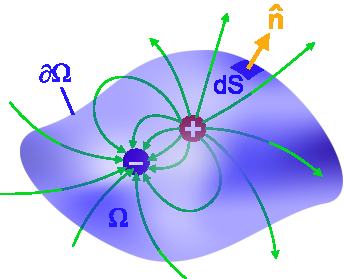
\includegraphics[width=.4\linewidth]{papers/kugel/figures/flux}}
  \caption{
    \label{kugel:fig:eeg}
  }
\end{figure}

To start, we will look at an application that is from the field of medicine:
electroencephalography. The \emph{electroencephalogram} (EEG) is a measurement
of the electrical field on the scalp, which shows the brain's activity, and is
used in many fields of research such as neurology and cognitive psychology.  The
measurement is done by wearing a cap that contains a number of evenly
distributed electrodes, each of which measures the electric potential (voltage)
at their location (figure \ref{kugel:fig:eeg-electrodes}).  To see how this will
relate to the spherical harmonics, we will first quickly recap a bit of physics,
electrodynamics to be precise.

In section \ref{kugel:sec:construction:eigenvalue} we have shown that the
spherical harmonics arise from the surface spherical Laplacian operator, whose
origin we did not consider too much, which is how mathematicians do their work.
On the contrary, physicists usually do the opposite and start by discussing what
is happening, since variables and functions represent physical quantities. So,
we will quickly remind that the Laplacian operator does the following to an
electric potential $\phi$:
\begin{equation*}
  \nabla^2 \phi
  = \nabla \cdot \nabla \phi
  = \nabla \cdot \mathbf{E}
  = \rho / \varepsilon
  \iff
  \iiint_\Omega \nabla \cdot \mathbf{E} \, dv
  = \iint_{\partial \Omega} \mathbf{E} \cdot d\mathbf{s}
  = \Phi / \varepsilon.
\end{equation*}
Put into words: on the left we have the differential form, where we recall that
the Laplacian (which is a second derivative) is the divergence of the gradient.
Unpacking the notation we first see that we have the gradient of the potential,
which is just the electric field $\mathbf{E}$, and then the divergence of said
electric field is proportional to the charge density $\rho$. So, the Laplacian
of the electric potential is the charge density! For those that are more
familiar with the integral form of Maxwell's equation, we have also included an
additional step using the divergence theorem, which brings us to the electric
Flux, which by Gauss' law (shown in the iconic\footnote{Every electrical
engineer has seen this picture so many times that is probably burnt in their
eyes.} figure \ref{kugel:fig:eeg-flux}) is the net electric charge.

\subsection{Measuring Gravitational Fields}

\subsection{Quantisation of Angular Momentum}

% vim:ts=2 sw=2 et spell tw=80:
\section{Long Proofs}

Here, we will give the long and tedious proofs we skipped earlier.

\subsection{Legendre Polynomials} \label{kugel:sec:proofs:legendre}

\begin{proof}[Proof of lemma \ref{kugel:thm:legendre-poly}]
  It was stated that the polynomial function
  \begin{equation*}
    P_n(z) = \sum^{\lfloor n/2 \rfloor}_{k=0}
      \frac{(-1)^k}{2^n s^k!} \frac{(2n - 2k)!}{(n - k)! (n-2k)!} z^{n - 2k}
  \end{equation*}
  is the only finite solution of the Legendre equation
  \begin{equation}
    \label{kugel:eqn:legendre-bis}
    (1 - z^2)\frac{d^2 Z}{dz^2}
    - 2z\frac{d Z}{dz}
    + n(n + 1) Z(z) = 0,
  \end{equation}
  when $n \in \mathbb{Z}$ and $z \in [-1; 1]$. In order to prove this fact, we
  begin with the power series \emph{Ansatz}
  \begin{equation*}
    Z(x) = \sum_{k=0}^\infty a_k z^k,
    \quad\text{from which follows that}\quad
    \frac{dZ}{dz} = \sum_{k=0}^\infty k a_k z^{k-1}, \qquad
    \frac{d^2 Z}{dz^2} = \sum_{k=0}^\infty k (k-1) a_k z^{k-2}.
  \end{equation*}
  Since the power series method converges only up to the nearest singularity,
  which is at $z=1$ (and $z=-1$), we shall remark that we will find a solution
  only for $|z|<1$. Using the \emph{Ansatz} the Legendre equation
  \eqref{kugel:eqn:legendre-bis} can be rewritten as
  \begin{align}
    0 &= (1-z^2) \sum_{k=0}^\infty k (k-1) a_k z^{k-2}
      - 2z\sum_{k=0}^\infty k a_k z^{k-1}
      + n(n+1)\sum_{k=0}^\infty a_k z^k \nonumber \\
    &= \sum_{k=0}^\infty k (k-1) a_k z^{k-2}
      - \sum_{k=0}^\infty k (k-1) a_k z^{k}
      - 2z\sum_{k=0}^\infty k a_k z^{k-1}
      + n(n+1)\sum_{k=0}^\infty a_k z^k. \label{kugel:eqn:legendre-ansatz}
  \end{align}
  Considers that by shifting the index $k$ in the sum of first term
  \begin{equation*}
    \sum_{k=0}^\infty k (k-1) a_k z^{k-2}
    = \sum_{k=-2}^\infty (k+2)(k+1) a_{k+2} z^k
    = \sum_{k=0}^\infty (k+2)(k+1) a_k z^k,
  \end{equation*}
  since when $k = -1$ or $-2$ the summand is zero. This means that
  \eqref{kugel:eqn:legendre-ansatz} becomes
  \begin{align*}
    \sum_{k=0}^\infty &(k+1)(k+2) a_{k+2} z^{k}
      - \sum_{k=0}^\infty k (k-1) a_k z^{k}
      - 2\sum_{k=0}^\infty k a_k z^k
      + n(n+1)\sum_{k=0}^\infty a_k z^k \nonumber \\
    &= \sum_{k=0}^\infty \big[
      (k+1)(k+2) a_{k+2}
      - k (k-1) a_k
      - 2 k a_k
      + n(n+1) a_k
    \big] z^k \stackrel{!}{=} 0,
  \end{align*}
  which is equivalent to saying that
  \begin{equation*}
    (k+1)(k+2) a_{k+2} - k (k-1) a_k - 2 k a_k + n(n+1) a_k = 0,
  \end{equation*}
  so we can derive a recurrence relation for $a_{k+2}$:
  \begin{equation}
    \label{kugel:eqn:coeff-recursion}
    a_{k+2} = \frac{k (k-1) - 2 k + n(n+1)}{(k+1)(k+2)}a_k
    = \frac{(k-n)(k+n+1)}{(k+2)(k+1)}a_k.
  \end{equation}
  Following the relation \eqref{kugel:eqn:coeff-recursion}, if we want to
  compute $a_6$ we have
  \begin{align*}
    a_{6} = -\frac{(n-4)(n+5)}{6\cdot 5} a_4
      &= \left( -\frac{(n-4)(5+n)}{6 \cdot 5} \right)
         \left( -\frac{(n-2)(n+3)}{4 \cdot 3} \right) a_2 \\
      &= \left( -\frac{(n-4)(n+5)}{6 \cdot 5} \right)
         \left( -\frac{(n-2)(n+3)}{4 \cdot 3} \right)
         \left( -\frac{n(n+1)}{2 \cdot 1} \right)  a_0 \\
      &= -\frac{(n+5)(n+3)(n+1)n(n-2)(n-4)}{6!} a_0.
  \end{align*}
  One can generalize this relation for the $i$-th even ($i = 2k$) coefficient
  and obtain
  \begin{equation*}
    a_{2k} = (-1)^k \frac{(n+(2k-1))(n+(2k-1)-2)
      \hdots (n-(2k-2)+2)(n-(2k-2))}{(2k)!}a_0,
  \end{equation*}
  and a similar expression can also be written for the odd coefficients
  $a_{2k-1}$. In the latter case, the equation starts from $a_1$ and to find the
  pattern we can write the recursion for an odd coefficient, for example for
  $a_7$:
  \begin{align*}
    a_{7} = -\frac{(n-5)(n+6)}{7\cdot 6} a_5
      &= \left( -\frac{(n-5)(n+6)}{7 \cdot 6} \right)
         \left( -\frac{(n-3)(n+4)}{5 \cdot 4} \right) a_3 \\
      &= \left( -\frac{(n-5)(n+6)}{7 \cdot 6} \right)
         \left( -\frac{(n-3)(n+4)}{5 \cdot 4} \right)
         \left( -\frac{(n-1)(n+2)}{3 \cdot 2} \right) a_1 \\
      &= -\frac{(n+6)(n+4)(n+2)(n-1)(n-3)(n-5)}{7!} a_1.
  \end{align*}
  As before, we can generalize this equation for the $i$-th odd ($i = 2k+1$)
  coefficient and get
  \begin{equation*}
    a_{2k+1} = (-1)^k \frac{(n + 2k)(n+2k-2)
      \hdots (n-(2k-1)+2)(n-(2k-1))}{(2k+1)!} a_1.
  \end{equation*}
  Now, if we let
  \begin{align*}
    Z_\text{e}^K(z) &:=
      \sum_{k=0}^K(-1)^k \frac{
        (n+(2k-1))(n+(2k-1)-2) \hdots
        \colorbox{red!20}{$(n-(2k-2)+2)(n-(2k-2))$}
      }{(2k)!} z^{2k}, \\
    Z_\text{o}^K(z) &:=
      \sum_{k=0}^K(-1)^k \frac{
        (n + 2k)(n+2k-2)\hdots \colorbox{blue!20}{$(n-(2k-1)+2)(n-(2k-1))$}
      }{(2k+1)!} z^{2k+1},
  \end{align*}
  we have a solution to the Legendre equation \eqref{kugel:eqn:legendre-bis},
  which can be written as
  \begin{equation} \label{kugel:eqn:legendre-powerseries}
    Z(z) = \lim_{K \to \infty} \left[
      a_0 Z_\text{e}^K(z) + a_1 Z_\text{o}^K(z)
    \right].
  \end{equation}
  However, as mentioned earlier this power series only converges for $|z| < 1$,
  but (for our application in the spherical harmonics) we want convergence for
  $|z| \leq 1$. This can only happen in one case: when the power series becomes
  \emph{finite}, i.e. a polynomial. To show that this happens, we analyze the
  colored parts separately:
  \begin{itemize}
    \item[\textcolor{red!80!black}{\textbullet}]
      Suppose that $n = n_0$ is an even integer. Then in the red part, for some
      value of $k=k_0$, it will happen that
      \begin{equation*}
        n_0-(2k_0-2)=0
        \iff
        n_0 = 2 k_0 - 2.
      \end{equation*}
      From that point on, given the recursive nature of
      \eqref{kugel:eqn:coeff-recursion}, all the subsequent coefficients will
      also be 0, making the sum finite.

    \item[\textcolor{blue!80!black}{\textbullet}]
      Suppose that $n=n_0$ is an odd integer. Then as before, in the blue part a
      specific value of $k=k_0$ will follow the following relation:
      \begin{equation*}
        n_0-(2k_0-1)=0
        \iff
        n_0 = 2k_0 - 1.
      \end{equation*}
      And from that point on, for the same reason as before, all the subsequent
      coefficients will also be 0, making the sum finite.
  \end{itemize} 

  Thus, we can see that if $n \in \mathbb{Z}$ the sum will always become finite,
  which is exactly what we want. Now, whichever the case notice that the
  polynomial will always be of degree $n$. We can use this fact to write a
  single expression that contains both the odd and even cases by unfolding the
  recursion \eqref{kugel:eqn:coeff-recursion} backwards. That is, instead of
  starting with $a_0$ to compute $a_2$, or with $a_1$ to compute $a_3$ and go
  on, we use $a_n$ and go backwards and write the solution as
  \begin{equation*}
    Z(z) = a_n z^n + a_{n-2} z^{n-2} + a_{n-4} z^{n-4} 
      + a_{n-6} z^{n-6} + \hdots +
      \begin{cases} 
        a_1 z, \quad &\text{if } n \text{ is odd} \\ 
        a_0, \quad  &\text{if } n \text{ is even} 
      \end{cases}
      = \sum_{k=0}^{\lfloor n/2 \rfloor} a_{n-2k}z^{n-2k}.
  \end{equation*}
  Therefore, we need to find how to compute $a_{n - 2k}$ starting from $a_n$.
  The game is like before to find a pattern, so
  \begin{align*}
    a_{n-2} &= -\frac{n(n-1)}{2(2n-1)}a_n, &
    a_{n-4} &= -\frac{(n-2)(n-3)}{4(2n-3)}a_{n-2}
    = \left(
        -\frac{(n-2)(n-3)}{4(2n-3)}
      \right) \left(
        -\frac{n(n-1)}{2(2n-1)}
      \right) a_n,
  \end{align*}
  and in general 
  \begin{equation*}
    a_{n-2k} = (-1)^k \frac{
      n(n-1)(n-2)(n-3) \cdots (n-2k+1)
    }{
      2 \cdot 4 \cdots 2k(2n-1)(2n-3) \cdots (2n-2k+1)
    } a_n.
  \end{equation*}
  To clean up this expression, we use
  \begin{equation*}
    n(n-1)(n-2)(n-3) \hdots (n-2k+1)
    = \frac{n!}{(n-2k)!}
  \end{equation*}
  in the part of the denominator
  \begin{align*}
    (2n-1) & (2n-3) \cdots (2n-2k+1) = \frac{
        2n(2n-1)(2n-2)(2n-3) \cdots (2n-2k+1)
      }{
        2n(2n-2)(2n-4)(2n-6) \cdots (2n-2k+2)
      }
      \\
      &= \frac{
        \frac{(2n)!}{(2n-2k)!}
      }{
        2^k n(n-1)(n-2)(n-3) \cdots (n-k+1)
      }
      = \frac{
        \frac{(2n)!}{(2n-2k)!}
      }{
        2^k \frac{n!}{(n-k)!}
      }
      = \frac{(n-k)!(2n)!}{n!(2n-2k)!2^k},
  \end{align*}
  and then since $2 \cdot 4 \cdots 2k = 2^r 1\cdot2 \cdots r = 2^r r!$, we
  obtain
  \begin{equation*}
    Z(x) = \sum_{k=0}^{\lfloor n / 2\rfloor}
      \underbrace{
        (-1)^k \frac{(n!)^2(2n-2k)!}{k!(n-2k)!(n-k)!(2n)!} a_n
      }_{a_{n-2k}} z^{n-2k},
  \end{equation*}
  which holds for any value of $a_n$. By letting
  \begin{equation*}
    a_{n} := \frac{(2n)!}{2^n (n!)^2},
  \end{equation*}
  the \emph{Legendre polynomials}
  \begin{equation}
    P_n(z) := \sum_{k=0}^{\lfloor n/2 \rfloor}
      (-1)^k \frac{(2n-2k)!}{2^n k! (n-k)!(n-2k)!} z^{n-2k} 
  \end{equation}
  emerges.
\end{proof}

\subsection{Associated Legendre Equation}
\label{kugel:sec:proofs:associated-legendre}

\begin{proof}[Proof of lemma \ref{kugel:thm:extend-legendre}]
  We want to show that if $Z_n(z)$ is a solution of the Legendre equation,
  \begin{equation} \label{kugel:eqn:legendre-bis}
    (1 - z^2)\frac{d^2 Z}{dz^2}
    - 2z\frac{d Z}{dz}
    + n(n + 1) Z(z) = 0,
  \end{equation}
  then
  \begin{equation*}
    Z^m_n(z) = (1 - z^2)^{m/2} \frac{d^m}{dz^m}Z_n(z)
  \end{equation*}
  solves the associated Legendre equation 
  \begin{equation*}
    (1 - z^2)\frac{d^2 Z}{dz^2}
    - 2z\frac{d Z}{dz}
    + \left( n(n + 1) - \frac{m^2}{1 - z^2} \right) Z(z) = 0.
  \end{equation*}
  To begin, we start by differentiating $m$ times \eqref{kugel:eqn:legendre-bis}
  (which is satisfied $Z(z)$), obtaining
  \begin{equation} \label{kugel:eqn:legendre-mderiv}
    \frac{d^m}{dz^m}\left[
      (1-z^2)\frac{d^2Z}{dz^2}
    \right]
    -2 \frac{d^m}{dz^m}\left[ z\frac{dZ}{dz} \right]
    + n(n+1)\frac{d^m}{dz^m}Z = 0.
  \end{equation}
  Since the notation is becoming cumbersome, we will define a new notation for
  derivatives:
  \begin{equation*}
    \frac{d}{dz} = \partial, \quad \text{and also} \quad
    \frac{d^k}{dz^k} = \partial^k.
  \end{equation*}
  \emph{Leibniz's theorem} states, that if we want to differentiate $m$ times a
  multiplication of two functions, we can use the binomial coefficients to build
  up a sum:
  \begin{equation*} %\label{kugel:eqn:leibniz}
    \partial^m \, (u \cdot v)
      = \sum_{i=0}^m \binom{n}{i} \, \partial^{m-i} u \, \partial^i v
  \end{equation*}
  By using the above in \eqref{kugel:eqn:legendre-mderiv}, we obtain
  \begin{align}
    0 &= \sum_{i=0}^m \underbrace{
      \binom{n}{i} \, \partial^{m-i} (1-z)^2 \, \partial^i Z(z)
    }_{\text{equals 0 when } m-i > 2}
    - 2 \sum_{i=0}^m \underbrace{
      \binom{n}{i} \, \partial^{m-i} z \, \partial^i Z(z)
    }_{\text{equals 0 when } m-i > 1}
    - n(n+1) \partial^m Z(z)
    \nonumber \\
    &= (1-z^2) \partial^{m+2} Z(z)
    + \partial (1-z^2) \partial^{m+1} Z(z)
    + \frac{m(m+1)}{2} \partial^2 (1-z^2) \partial^m Z(z)
    \nonumber \\
    &\qquad - 2 \left(
      z \partial^{m+1} Z(z)
      + m\partial z \partial^m Z(z)
    \right)
    + n(n+1) \partial^m Z(z)
    \nonumber \\
    &= (1-z^2) \partial^2 \partial^m Z(z)
    - 2z \partial \partial^m Z(z)
    + \bigl[ n(n + 1) - m(m-1) - 2m \bigr] \partial^m Z(z).
    \label{kugel:eqn:legendre-leibniz}
  \end{align}
  % old notation
  % \begin{align}
  %   (1-z^2)\frac{d^{m+2}Z}{dz^{m+2}}
  %     &+ m \frac{d}{dz}(1-z^2)\frac{d^{m+1}Z}{dz^{m+1}}
  %     + \frac{m(m-1)}{2}\frac{d^{2}}{dz^{2}}(1-z^2)\frac{d^{m}Z}{dz^{m}}
  %     \nonumber \\
  %     &\qquad \qquad \qquad \qquad \qquad
  %     + n(n+1)\frac{d^m{}Z}{dz^{m}}
  %     -2\left(
  %       z\frac{d^{m+1}Z}{dz^{m+1}}
  %       + m\frac{d}{dz}z\frac{d^{m}Z}{dz^{m}}
  %     \right)
  %     \nonumber \\
  %   &= (1-z^2)\frac{d^{m+2}Z}{dz^{m+2}}
  %     -2z(m+1)\frac{d^{m+1}Z}{dz^{m+1}}
  %     +(n(n+1)-m(m-1)-2m)\frac{d^{m}Z}{dz^{m}}
  %     =0. \label{eq:auz_3}
  % \end{align}
  Now, we can define a new function
  \begin{equation*}
    Z^m(z) = (1-z^2)^{m/2} \partial^m Z(z)
    \iff
    \partial^m Z(z) = (1-z^2)^{-m/2} Z^m(z),
  \end{equation*}
  and we claim that it is a solution to the associated Legendre equation. To
  show that, we insert it in \eqref{kugel:eqn:legendre-leibniz}, which gives
  \begin{align*}
    0 &= (1-z^2) \partial^2 \bigl[ (1-z^2)^{-m/2} Z^m(z) \bigr]
    - 2z\partial \bigl[ (1-z^2)^{-m/2} Z^m(z) \bigr]
    \\
    &\qquad + \bigl[ n(n + 1) - m(m-1) - 2m \bigr] (1-z^2)^{-m/2} Z^m(z).
  \end{align*}
  We will analyze the messy right hand side one term at the time. With a bit of
  effort one can show that
  \begin{align*}
    \partial \bigl[ (1-z^2)^{-m/2} Z^m(z) \bigr]
      &=
  \end{align*}
  and differentiating again
  \begin{align*}
    \partial^2 \bigl[ (1-z^2)^{-m/2} Z^m(z) \bigr]
      &= (1-z^2)^{-m/2-1} \partial^2 Z^m(z)
        + 2mz(1-z^2)^{-m/2 -1} \partial Z^m(z) \\
        &\qquad + m (1-z^2)^{-m/2-1} Z^m(z) 
        + m z(m+2)(1-z^2)^{-m/2} Z^m(z).
  \end{align*}
  The goal now is to compute the two terms 
  \begin{align*}
    \frac{d^2}{dx^2}[\hat{y}_m(1-x^2)^{-\frac{m}{2}}] &=  \frac{d^2\hat{y}_m}{dx^2} (1-x^2)^{-\frac{m}{2}} + \frac{d\hat{y}_m}{dx}\frac{m}{2}(1-x^2)^{-\frac{m}{2}-1}2x \\
    &+ m\left( \frac{d\hat{y}_m}{dx} x (1-x^2)^{-\frac{m}{2}-1} + \hat{y}_m (1-x^2)^{-\frac{m}{2}-1} - \hat{y}_m x (-\frac{m}{2}-1)(1-x^2)^{-\frac{m}{2}} 2x\right) \\
    &= \frac{d^2\hat{y}_m}{dx^2} (1-x^2)^{-\frac{m}{2}} + \frac{d\hat{y}_m}{dx}mx (1-x^2)^{-\frac{m}{2}-1} + m\frac{d\hat{y}_m}{dx}x (1-x^2)^{-\frac{m}{2}-1}\\
    &+ m\hat{y}_m  (1-x^2)^{-\frac{m}{2}-1} + m\hat{y}_m x^2(m+2)(1-x^2)^{-\frac{m}{2}-2}
  \end{align*}
  and
  \begin{align*}
    \frac{d}{dx}[\hat{y}_m(1-x^2)^{-\frac{m}{2}}] &= \frac{d\hat{y}_m}{dx}(1-x^2)^{-\frac{m}{2}} + \hat{y}_m\frac{m}{2}(1-x^2)^{-\frac{m}{2}-1}2x \\
    &= \frac{d\hat{y}_m}{dx}(1-x^2)^{-\frac{m}{2}} + \hat{y}_mm(1-x^2)^{-\frac{m}{2}-1}x,
  \end{align*}
  to use them in Eq.\eqref{eq:2st_subs}, obtaining
  \begin{align*}
    (1-x^2)\biggl[\frac{d^2\hat{y}_m}{dx^2} (1-x^2)^{-\frac{m}{2}} &+ \frac{d\hat{y}_m}{dx}mx (1-x^2)^{-\frac{m}{2}-1} + m\frac{d\hat{y}_m}{dx}x (1-x^2)^{-\frac{m}{2}-1} \\ 
    &+ m\hat{y}_m  (1-x^2)^{-\frac{m}{2}-1} + m\hat{y}_m x^2(m+2)(1-x^2)^{-\frac{m}{2}-2}\biggr] \\
    &-2(m+1)x\left[  \frac{d\hat{y}_m}{dx}(1-x^2)^{-\frac{m}{2}} + \hat{y}_mm(1-x^2)^{-\frac{m}{2}-1}x \right] \\
    &+ (n(n+1)-m(m+1))\hat{y}_m(1-x^2)^{-\frac{m}{2}}=0.\\
  \end{align*}
  We can now divide by $(1-x^2)^{-\frac{m}{2}}$, obtaining
  \begin{align*}
    (1-x^2)\biggl[\frac{d^2\hat{y}_m}{dx^2} &+ \frac{d\hat{y}_m}{dx}mx (1-x^2)^{-1} + m\frac{d\hat{y}_m}{dx}x (1-x^2)^{-1} + m\hat{y}_m  (1-x^2)^{-1} + m\hat{y}_m x^2(m+2)(1-x^2)^{-2}\biggr] \\
    &-2(m+1)x\left[  \frac{d\hat{y}_m}{dx} + \hat{y}_mm(1-x^2)^{-1}x \right] + (n(n+1)-m(m+1))\hat{y}_m\\
    &= \frac{d^2\hat{y}_m}{dx^2} + \frac{d\hat{y}_m}{dx}mx + m\frac{d\hat{y}_m}{dx}x + m\hat{y}_m + m\hat{y}_m x^2(m+2)(1-x^2)^{-1} \\
    &-2(m+1)x\left[  \frac{d\hat{y}_m}{dx} + \hat{y}_mm(1-x^2)^{-1}x \right] + (n(n+1)-m(m+1))\hat{y}_m\\
  \end{align*}
  and collecting some terms
  \begin{equation*}
    (1-x^2)\frac{d^2\hat{y}_m}{dx^2} - 2x\frac{d\hat{y}_m}{dx} + \left( -x^2 \frac{m^2}{1-x^2} + m+n(n+1)-m(m+1)\right)\hat{y}_m=0.
  \end{equation*}
  Showing that 
  \begin{align*}
    -x^2 \frac{m^2}{1-x^2} + m+n(n+1)-m(m+1) &= n(n+1)- m^2 -x^2 \frac{m^2}{1-x^2} \\
    &= n(n+1)- \frac{m}{1-x^2}
  \end{align*}
  implies $\hat{y}_m(x)$ being a solution of Eq.\eqref{kugel:eq:associated_leg_eq}
\end{proof}

\subsection{Orthogonality}


\printbibliography[heading=subbibliography]
\end{refsection}
\end{otherlanguage}
